\documentclass[12pt,oneside,letterpaper,hyphens]{memoir}
\usepackage[style=ieee,citestyle=numeric-comp,sorting=nty,backend=biber]{biblatex}
\usepackage{todonotes}                                      % Temp

\usepackage{hyperref}                                       % Make table of contents clickable, allow URLs
\usepackage{textcomp}                                       % For tilde
\usepackage{graphicx}                                       % Images
\usepackage{array}                                          % Table spacing
\usepackage{ragged2e}                                       % Left align table text
\usepackage{caption}                                        % Use to create the \repeatcaption command
\usepackage{float}                                          % Image placement
\usepackage[fit]{truncate}                                  % Truncate section names in the header
\usepackage{charter}                                        % Charter font
% \usepackage[]{cabin}                                      % Cabin font
% \usepackage{tgpagella}                                      % Gyre Pagella font
% \usepackage{bookman}                                        % Bookman font
\usepackage[acronym,noredefwarn]{glossaries}                % Glossary, acronyms list, etc
\usepackage{acronym}                                        % Acronym specific things
\usepackage{glossary-mcols}                                 % Multi-column glossary or acronyms list
\usepackage{xparse}                                         % Better parsing for macros
\usepackage[detect-all]{siunitx}                            % SI unit formatting
\usepackage{appendix}                                       % Appendices
\usepackage{minted}                                         % Code!
\usepackage{amsmath}                                        % Math
\usepackage{caption}                                        % Captions for formulas
\usepackage{microtype}                                      % General typography improvements
\usepackage[english]{babel}                                 % For "fancy" quotes
\usepackage[autostyle, english=american]{csquotes}          % Same
\usepackage{wrapfig}                                        % Figures wrapped by text
\usepackage{cleveref}                                       % Improved cross references

\MakeOuterQuote{"}                                          % For fancy quotes
\hypersetup{colorlinks=true,                                % Blue hyperlinks, everything else black
            urlcolor=blue,
            citecolor=black,
            linkcolor=black}
% \renewcommand\familydefault{\sfdefault}                     % Sans serif
\newcommand{\textapprox}{\raisebox{0.1ex}{\texttildelow}}   % Add a ~ character for approximate values
\newcommand{\repeatcaption}[2]{                             % \repeatcaption command for reusing figures
  \renewcommand{\thefigure}{\ref{#1}}
  \captionsetup{list=no}
  \caption{#2 (repeated from page \pageref{#1})}
}

% Fix code centering
\RecustomVerbatimEnvironment{Verbatim}{BVerbatim}{}

% 1 in margins
\setulmarginsandblock{1in}{1in}{*}
\setlrmarginsandblock{1in}{1in}{*}
\checkandfixthelayout

% Head and chapter styles
% \setlength\prechapterprecisshift{0pt}
% \headstyles{komalike}

% Good:
\chapterstyle{madsen}
% \chapterstyle{ell}

% Okay:
% \chapterstyle{veelo}
% \chapterstyle{dash}
% \chapterstyle{verville}
% \chapterstyle{dowding}
% \chapterstyle{southall}
% \chapterstyle{demo2}
% \chapterstyle{chappell}
% \chapterstyle{ger}


% Show subsection numbers and entries in TOC
\setsecnumdepth{subsection}
\maxtocdepth{subsection}

%% Turning these on shrinks whitespace MASSIVELY.
% \setbeforesecskip{0.35em}
% \setaftersecskip{0.2em}
% \setbeforesubsecskip{0.5em}
% \setaftersubsecskip{.1em}
% \setbeforeparaskip{0.5em}
% \setlength{\beforechapskip}{0.5em}
% \setlength{\afterchapskip}{0.3em}
% \setlength{\belowcaptionskip}{-0.1em}

% Macro for acronyms with description
\let\newacronymsaved\newacronym
% \def\?#1{}
\RenewDocumentCommand\newacronym{mmmg}{
    % Fuck all ye who enter here
    \expandafter\newcommand\expandafter{\csname #1\endcsname}[0]{\gls{#1}\,}
    \expandafter\newcommand\expandafter{\csname #1s\endcsname}[0]{\glspl{#1}\,}
    \expandafter\newcommand\expandafter{\csname #2\endcsname}[0]{\Gls{#1}\,}
    \expandafter\newcommand\expandafter{\csname #2s\endcsname}[0]{\Glspl{#1}\,}
    \IfNoValueTF{#4}{
        \newacronymsaved{#1}{#2}{#3}
    } {
        \newglossaryentry{#1}{
                            type=\acronymtype, 
                            name={#2}, 
                            description={#3}, 
                            first={#3 (#2)\glsadd{#1-gls}}, 
                            plural={⟨#2⟩\glspluralsuffix},
                            firstplural={⟨#3⟩\glspluralsuffix\space (⟨#2⟩\glspluralsuffix)},
                            see=[Glossary:]{#1-gls}}
        \newglossaryentry{#1-gls}{name={#2}, description={#4. \textit{See pgs}}}
    }
}

% Some new units
\DeclareSIUnit{\dollar}{\$}
\DeclareSIUnit{\bit}{b}
\DeclareSIUnit{\byte}{B}

% Captioned equation (formula) environment
\DeclareCaptionType{formula}[][]
\captionsetup[formula]{name=Formula,labelformat=default,font={it,small},margin=0.5in}

\newmintedfile[inputsql]{postgresql}{
    linenos,
    autogobble,
    breaklines,
    fontsize=\footnotesize,
}


\graphicspath{{images/}}

\title{\scshape Evaluating Internet Connectivity in the United States}
\author{Samuel Goldman, Evan Goldstein, Christopher Myers, David Vollum}
% \date{September 2019}

% Glossary info goes in the preamble
\makeglossaries

% Acronyms
% Follow the form: \newacronym{label}{ACRONYM}{expansion}
% Also: alphabetize!
\newacronym{anova}{ANOVA}{analysis of variance}
\newacronym{api}{API}{application programming interface}
\newacronym{aws}{AWS}{Amazon Web Services}
\newacronym{caida}{CAIDA}{Center for Applied Internet Data Analysis}
\newacronym{cdf}{CDF}{cumulative distribution function}
\newacronym{cors}{CORS}{cross-origin resource sharing}
\newacronym{csv}{CSV}{comma separated value}
\newacronym{cv}{CV}{coefficient of variation}
\newacronym{ddos}{DDoS}{distributed denial of service}
\newacronym{dns}{DNS}{domain name system}
\newacronym{dsl}{DSL}{digital subscriber line}
\newacronym{fcc}{FCC}{Federal Communications Commission}
\newacronym{gis}{GIS}{geographic information system}
\newacronym{gps}{GPS}{global positioning system}
\newacronym{html}{HTML}{Hypertext Markup Language}
\newacronym{http}{HTTP}{hypertext transfer protocol}
\newacronym{httpse}{HTTPS}{hypertext transfer protocol secure}
\newacronym{idw}{IDW}{inverse distance weighting}
\newacronym{ip}{IP}{internet protocol}
\newacronym{ipvs}{IPv6}{internet protocol version 6}
\newacronym{ipvf}{IPv4}{internet protocol version 4}
\newacronym{isp}{ISP}{internet service provider}
\newacronym{json}{JSON}{Javascript Object Notation}
\newacronym{kde}{KDE}{kernel density estimation}
\newacronym{mbps}{Mbps}{megabits per second}
\newacronym{mqp}{MQP}{major qualifying project}
\newacronym{ntp}{NTP}{Network Time Protocol}
\newacronym{ripe}{RIPE}{R\'eseaux IP Europ\'eens}
\newacronym{rtt}{RTT}{round trip time}
\newacronym{sdk}{SDK}{software development kit}
\newacronym{tcp}{TCP}{transmission control protocol}
\newacronym{tld}{TLD}{top level domain}
\newacronym{tls}{TLS}{transport layer security}
\newacronym{ttl}{TTL}{time-to-live}
\newacronym{acUrl}{URL}{uniform resource locator}
\newacronym{us}{US}{United States}
\newacronym{voip}{VoIP}{voice over internet protocol}
\newacronym{wpi}{WPI}{Worcester Polytechnic Institute}

% Acronyms with definitions
% Follow the form: \newacronym{label}{ACRONYM}{expansion}{description}. Description appears in glossary only.
 \newacronym{cdn}{CDN}{content delivery network}{A Content Distribution Network (CDN), sometimes called a Content Delivery Network, is a network of proxy servers that form a kind of cache used to enhance delivery of content to internet users. Although helpful for internet users, they complicate measurements of connectivity to websites \textit{actually} connecting to the site's servers}
 
 \newacronym{icmp}{ICMP}{internet control message protocol}{Internet Control Message Protocol (ICMP) is a protocol designed for error reporting and other utility purposes across the internet, typically used most by routers and other intermediary devices}
 
%  \newacronym{cv}{CV}{coefficient of variance}{Coefficients of variance (CVs) are calculated by dividing the standard deviation of a data set by its mean. CVs are dimensionless values that can be judged independent of the data set, making them useful for gauging the spread of any data set. The lower the CV, the lower the spread of the data and the better the quality}
 
 \newacronym{etl}{ETL}{extract, transform, load}{ETL is a generic procedure for extracting data, transforming it into a more useful format, and loading it into a large volume storage system, such as a database. The term closer describes an architecture rather than a specific algorithm}
 
 \newacronym{ecc}{EC2}{Amazon Elastic Compute Cloud}{EC2 is a service from Amazon Web Services that provides virtual machines in the cloud for general-purpose or task optimized work. EC2 can be configured for different performance and pricing classes, as well as complex auto-scaling schemes or virtual private cloud setups}
 

% Glossary entries -- these should be more detailed.
% Follow the form: \newglossaryentry{LABEL}{name={NAME} description={YOUR TEXT HERE}}
% \newglossaryentry{favicon}{
%     name={favicon},
%     description={Favicons are small identifying images, typically logos or relevant UI elements, that most websites provide for browsers to place on tabs and bookmarks. Favicons are stored as .ico files (icons) and are either 16x16, 32x32, or 48x48. This small size makes them ideal for testing connection \rtt from a browser}
% }

% \newglossaryentry{backbone}{
%     name={internet backbone},
%     description={Internet backbone infrastructure consists of very high speed principal data routes and the connected major computer networks and core routers. For any trip of serious distance (likely most connections, unless you happen to have a data center in your backyard), packets will inevitably pass through some element of the internet backbone}
% }

% \newglossaryentry{traceroute}{
%     name={traceroute},
%     description={A traceroute is a technique that shows the full path data takes to get from your computer to a remote server, and how long it takes to get to each server along the way. Traceroutes leverage \icmp and specifically-set \ttl values to inciteintermediate servers to respond with an \icmp packet indicating the data packet's \ttl has expired -- thereby giving away the server's presence along the route}
% }


% Bibliography goes in the preamble
\bibliography{references}

% UNCOMMENT TO DISCOURAGE WILLS FROM PRINTING
% \pagecolor[rgb]{0, 0, 0}
% \color[rgb]{1,1,1}

\begin{document}
    %%%%%%%%%%%%%%%%%%%%
    %%% FRONT MATTER %%%
    %%%%%%%%%%%%%%%%%%%%
    
    % Title page
    \frontmatter
    \pagenumbering{gobble}
    \noindent\begin{minipage}{0.1\textwidth}
    \colorrule{0.25in}{\textheight}{WPIRed}
\end{minipage}
\begin{minipage}{0.9\textwidth}
    \begin{center}
        \Huge\noindent Evaluating Internet Connectivity in the United States
        \vspace{0.75in}
        
        \missingfigure{Some kind of title page picture}
        % \includegraphics[width=0.5\columnwidth]{img/final_clamp.png}
    \end{center}
    \vspace{1in}
    \begin{minipage}{\textwidth}    
        \begin{flushright}
            \includegraphics[width=0.5\textwidth]{WPI_logo.png} 
        \end{flushright}
    \end{minipage}
    \noindent\begin{minipage}{0.5\textwidth}
        \small
        Samuel Goldman \\
        Evan Goldstein \\
        Christopher Myers \\
        David Vollum
    \end{minipage}
    \begin{minipage}{0.5\textwidth}
        \begin{flushright}
            \small
            Worcester Polytechnic Institute \\
            Department of Computer Science\\
            February 2019
        \end{flushright}
    \end{minipage}
\end{minipage}
   
    % Abstract
    \begin{abstract}
We evaluated internet connectivity in the United States, drawn from different definitions of connectivity and different methods of analysis. Using DNS cache manipulation, traceroutes, and a crowdsourced “web ping” method we identify patterns in connectivity that correspond to higher population or coastal regions of the US. We analyze the data for quality strengths and shortcomings, establish connectivity heatmaps, state rankings, and statistical measures of the data. We give comparative analyses of the three methods and present suggestions for future work building off this report.
\end{abstract}
    \newpage
    
    % Table of contents, list of figures
    \pagenumbering{roman}
    % \listoftodos\newpage
    \tableofcontents\newpage
    \listoffigures\newpage
    \listofcodesnippets\newpage
    \listoftables\newpage
    
    % Switch to arabic page numbering, start headers, and one half spacing.
    % \pagenumbering{arabic}
    \pagestyle{headings}
    \mainmatter
    
    %%%%%%%%%%%%%%%%%%%%%%%%%%%
    %%% MAIN PAPER CONTENTS %%%
    %%%%%%%%%%%%%%%%%%%%%%%%%%%
    
    % TO ADD CONTENT:
    % Add a file under the text folder, put your stuff there, then \input it in the
    % spot where it should go. THIS MEANS YOU DON'T HAVE TO DEAL WITH ONE GIANT MANUSCRIPT!
    
    \chapter{Introduction}\label{sec:introduction}
    Internet access is an increasingly important part of the American economy and everyday life. Common tasks like applying for a job, keeping in touch with friends, and education all require internet connectivity. Major technology firms are often in the public spotlight, and common internet services can be found everywhere, such as music and video streaming, e-books, and shopping. In 2018 an industry group comprised of major technology firms estimated that the "internet sector" of the economy alone represented \$2.1 trillion a year, or about 10\% of the \us economy \cite{Shepardson2019a}.

Unfortunately, not all parts of the \us are as well connected as others, even by measures from simple personal anecdotes. For example, in rural areas the best connection frequently is not good enough to stream a movie, while driving just 45 minutes to a more urban area will yield a connection an order of magnitude better. Subjective measures like this are common everywhere across the \us, but there is little scientifically-rigorous or complete data available. For instance, the \fcc has a map of estimated broadband deployment \cite{FederalCommunicationsCommission}, but simple broadband deployment is not necessarily a good measure of how well connected people in those areas actually are.

To address these problems, we set out to gather and analyze as much data as possible on how well connected Americans are to the internet, using various means and measures. Our hypothesis is simple: although there may be some regional variations or "spottiness," there is a relationship between your location in the \us and what sort of internet service you can expect. We hypothesized that areas near each other are likely to have similar connectivity to one another, and that these similarities will form large-scale trends that should be visible on a map, interpretable by non-technical readers.

The end goal of our project was to find if such relationships exist, and if so, to conduct analyses on the data to make the differences between areas of the \us clear. An important quality of our work is that it should be scientifically rigorous and statistically valid -- that is, we should avoid systemic error and account for random error in our calculations -- so a great deal of effort was expended on ensuring the validity of our results.

The reminder of the report is organized into chapters as follows:

In \cref{sec:background} we present background information on the fundamentals of the internet, information relevant to our methods, and research conducted on prior works and attempts at measuring connectivity.

In \cref{sec:connectivity_defs} we rely upon collected background research to define metrics for internet connectivity. These are not limited to traditional metrics used by consumers (such as speed), instead taking a more expansive approach.

\Cref{sec:methods} describes a brief overview of our three main methods for collecting \& analyzing data on internet connectivity. We also present a brief overview of the statistical methods used, and an explanation of methods that were considered but ultimately rejected.

\Crefrange{sec:caida}{sec:dns} present detailed methods of the design, implementation, and analysis for each of our three methods for collecting data. Their analyses differ since each data set is somewhat different, but the fundamentals (e.g. definitions of connectivity) remain largely the same.

\Cref{sec:comparative_analyses} contains our comparative analysis of the results of the three data analyses. We present overall conclusions drawn from the data, in both assertions we are confident of and matters we are uncertain of.

Finally, in \cref{sec:future_work} we suggest ideas for future projects to follow up on, drawing from shortcomings noted in our methods and the unpursued methods explained in \cref{sec:methods}.

    
    \acresetall
    \newpage
    \chapter{Background}\label{sec:background}
    This chapter presents an overview of the underpinnings of the internet and elements critical to understanding how our analyses work. The below sections are not intended to be comprehensive texts, only mostly-conceptual overviews of the fundamental principles of this report.

    \section{Internet Architecture}\label{sec:background_internet_architecture}

The internet is formed from a broad range of networks spread across the globe, connected together by very high speed links and data centers traditionally referred to as the "\textbf{backbone}." Although the networks are distributed, they do not form a true mesh network. Instead, data is generally routed through hierarchical networks. These start at the small, local level, and progress upwards (as needed, depending on the \isp's architecture) through increasingly larger networks as data is routed to its final destination, eventually repeating the process in reverse as packets approaches their destination server.

Since the internet takes a hierarchical format, end users are prone to experiencing the bottleneck that is the lowest tier networks they are connected to: their \isp, its parent network, and so on. As a result internet connections vary in all ways across the United States, with some areas receiving over 50 \mbps while others receive less than 1. 
    \section{Traceroutes}\label{sec:background_traceroutes}

A traceroute is a method for determining which servers are along a packet's route, and determining the \rtt to each of them. Most traceroute programs work using \icmp but in theory anything that uses \ip works.

Traceroutes hinge on the \ttl field of \ip packets, an eight-bit field that is decremented by one every time the packet is processed \cite{rfc791}. Typically this is set reasonably high so packets can take many hops to reach their destination, but low enough that if undeliverable they will eventually be discarded. Upon discard, most servers respond with an \icmp packet to the original host indicating \ttl expiry. This message is received by the machine running the traceroute, which uses the sender's \ip address and knowledge of the \ttl of the packet it sent out to place the server somewhere along the route. This process is visualized in \cref{fig:traceroute_diagram}.

\begin{figure}[h]
    \centering
    \missingfigure{Traceroutes diagram}
    \caption{Diagram of how traceroutes work}
    \label{fig:traceroute_diagram}
\end{figure}

The mechanics of a traceroute program are then a very simple procedure. With $i=1$ to start, an \icmp-based traceroute program follows the below:

\begin{enumerate}
    \item Send an \icmp ping with \TTL$=i$ to the destination server.
    \item If an \icmp \ttl-expired packet is received, mark the sender as hop $i$ along the route. If a timeout is reached, skip.
    \item If an \icmp ping response is received (i.e. the destination was reached), mark the destination server as the $i$-th hop and note the time it took to receive the packet.
    \item Increment $i$ by one and repeat from step 1.
\end{enumerate}

This process produces a list of servers along the route and their associated \rtts. A sample output from the aptly-named \texttt{traceroute} utility\footnote{\texttt{traceroute} and its variations can be found on virtually every system made in recent memory. Linux distributions and Windows machines ship with command-line tools \texttt{traceroute} and \texttt{tracert} respectively, while MacOS has its own dedicated GUI application as a system tool.} is shown in \cref{fig:sample_traceroute}. The \texttt{* * *} instances on lines 2 and 10 indicate that no response was received from these hops, so \texttt{traceroute} proceeded without them.

\begin{code}
\centering
\begin{minipage}{0.33\textwidth}
    \begin{minted}{text}
 1  192.168.1.1  16.529 ms
 2  * * *
 3  96.34.83.9  26.158 ms
 4  96.34.84.212  30.452 ms
 5  96.34.2.142  31.084 ms
 6  96.34.0.51  31.012 ms
 7  96.34.0.137  27.184 ms
 8  96.34.3.89  23.049 ms
 9  96.34.148.35  28.703 ms
10  * * *
11  108.170.246.33  26.405 ms
12  108.170.246.34  24.091 ms
13  172.217.164.142 24.720 ms
    \end{minted}
\end{minipage}
    \caption{Truncated output from \texttt{traceroute google.com}}
    \label{fig:sample_traceroute}
\end{code}

    \section{Speed Test}\label{sec:speed_test_background}

Speed tests are common measures used by consumers to figure out how "good" their internet connection is. The idea is simple -- connect to a website and try to transfer as much content as possible within some timeframe. The amount of data transferred can be used to calculate a data transfer speed in \Mbps, where higher is better. Examples include Ookla's aptly-named \url{speedtest.net}, or Netflix's \url{fast.com}.

In theory speed tests are a sound idea, since speed of data transfer is the most immediately obvious thing to a consumer. Connection speed dictates everything from how long it takes pages to load, to how long videos have to buffer, to how fast you can download files. In practice, though, speed testing is challenging and often inaccurate. In order to accurately measure speed, you must have a server receiving and sending test data with at \textit{least} the same speed as the summed connections of all of its users at any one time, posing an immediate performance challenge. Second, the measured connection is only the one between you and whatever data center the speed test server is located in, which may not represent your overall connectivity. Finally, \isps are doubtless familiar with speed test sites and have a serious motive to bias connections in favor of them, to trick their customers into thinking they have better internet than they actually do.

As a result of these combined factors, we decided against using traditional speed tests as any method for assessing internet connectivity.

    \section{Caching}\label{sec:background_caching}

RFC 7234 describes caching as the process of storing "cacheable responses in order to reduce the response time and network bandwidth consumption on future, equivalent requests" \cite{rfc7234}. Caches save frequently-used resources for a given amount of time to reduce the load on upstream resources, from the origin server to Internet infrastructure that provides service along the way. Several components of the Internet may contain caches: the user's browser, \cdns (see \cref{sec:background_cdns}), \dns servers, and others \cite{MozillaFoundation2019HTTPCaching}. These all work together to free up Internet bandwidth and provide a smoother experience to end users.

% Browser caching
Most (if not all) web browsers implement \http caching, saving commonly-used website resources locally \cite{Grigorik2019HTTPCaching}. For example, if users make frequent requests to \texttt{amazon.com}, a cache between Amazon's servers and their users may store a copy of Amazon's logo as it does not change frequently. When \texttt{amazon.com} then requests the logo, the browser's cache responds with the copy, preventing the request from going all of the way to Amazon's servers. This reduces network load that would normally be caused by the request. Of course, sometimes resources do change, so an origin server can give cacheable resources an expiration time after which the cache should validate the freshness resource before fulfilling the request \cite{rfc7234}. 

% CDN caching - not sure if this belongs, maybe just a brief overview before the dedicated CDN section.
Outside of the browser, web resources are often cached by \cdns. These networks are set up by companies that operate major websites and are intended to move the delivery of frequently accessed resources closer to end users, both in network and geographic terms. \cdns are discussed in more detail in \cref{sec:background_cdns}.

% DNS caching
Beyond caching resources that the end user sees and interacts with, other things, like \dns results, use caching as well. As discussed in more detail in \autoref{sec:background_dns}, recursive \dns servers retrieve requests from other \dns servers and often cache them for responding to future requests \cite{rfc1035}. Similar to the expiration time in HTTP caching, \dns caching has a \ttl that forces the \dns resolver to request a fresh answer.
    \section{Domain Name System}\label{sec:background_dns}
\dns, a key component of internet infrastructure and connectivity, is a hierarchical system responsible for converting domain names to \ip addresses. Domain names are human-readable names used to identify servers and websites. They are easier to remember than \ip addresses, and can point to more than one address depending on geographic location or load-balancing constraints to provide higher-performance access to websites for end-users. Domain names contain one or more parts called \textit{labels}, separated by dots. The rightmost label is the \tld (e.g. \texttt{com}, \texttt{org}, \texttt{net}, etc.). The \dns hierarchy tree subdivides into "zones," with each zone containing one or more domain names and sub-domains. Databases of domain names are maintained by \dns Name Servers, which resolve domains to \ip addresses  (\cref{fig:dns_resolution}). There are two types of name servers: authoritative and recursive.

\begin{wrapfigure}[18]{R}{0.4\textwidth}Beyond caching resources that the end user sees and interacts with, other things, like \dns results, use caching as well. As discussed in more detail in \autoref{sec:background_dns}, recursive \dns servers retrieve requests from other \dns servers and often cache them for responding to future requests \cite{rfc1035}. Similar to the expiration time  in HTTP caching, \dns caching has a \ttl that for


    \centering
    \includegraphics[width=0.4\textwidth]{images/other/dns_lookup_diagram.png}
    \caption{Diagram of DNS resolution \cite{Cloudflare2020a}}
    \label{fig:dns_resolution}
\end{wrapfigure}

\subsection{Authoritative Servers}
Authoritative servers are the primary source for the domain names within a given zone. When querying for any domain, the answer will ultimately come from the authoritative server for that domain. A \dns client can query an authoritative server directly, but it is more common that an authoritative server will be queried by a recursive server on behalf of a \dns client.

\subsection{Recursive Servers}
Recursive \dns servers work to find an \ip address for a client, so that the client does not have to do the leg work of searching through other \dns servers \cite{Cloudflarea}. \DNS resolvers use a predetermined upstream recursive \dns server, such as one provided by an \isp \cite{Oracle2010RecursiveWork}. This server then checks its cache and, if it has a valid answer, returns it. Otherwise, the server makes a series of iterative queries in order to find the requested name. 

Take for example, \texttt{www.google.com}. If the recursive server has no knowledge of any parts of the \acUrl, it will first query a pre-configured root \dns server for the authoritative server for the \texttt{.com} \tld. It will then query that server for \texttt{google.com}, then query the server provided from that request for \texttt{www.google.com} itself. At this point, the iterative component of the lookup is complete. At each stage of this process, the recursive server caches the results of its query, and assuming the \ttl has not expired, will use that cached value instead of making a fresh query. Finally, the recursive server then returns the \ip address it located, completing the recursive request from the user.

\paragraph{Public Recursive \dns Servers}
An important part of this project involves public recursive \dns servers. These servers are \dns servers configured to respond to requests from anyone. Whereas most \isp servers don't advertise their \dns servers to non-customers, public servers do. Some organizations, like Google and CloudFlare, provide public \dns services because they believe doing so improves the browsing experience for end users \cite{GoogleIntroductionDNS}. These provide the public with \dns options outside of their \isp and provide this project with an important set of geographically diverse servers.

    \section{Content Delivery Networks}\label{sec:background_cnds}
\textit{Assigned to: David}
Content delivery networks \cdn's are used by many popular websites across to the Internet to deliver content quickly and efficiently to its end users. Content Delivery Networks are made of data centers that are distributed across the world. These data centers are often located near large population centers, and ISP's network backbone. Some \cdn's are even run by the ISP itself, primarily to help alleviate strain on there infrastructure.  Content owners, such as Netflix or Reddit, pay Content Delivery Network providers to host there content on all of there servers around the world and therefor serve it efficiently to the end users. \cite{} One of the drawbacks of \cdn's it can often be difficult to update the data stored within them. As a result they are often used for static content that doesn't get updated very often, such as videos for Netflix or user content that is posted to Reddit. One example of a map can be seen below for Reddit. \todo add image for reddit to show their \cdn.
    \section{IP Geolocation \& Reverse Geocoding}\label{sec:background_geolocation}
Geolocation services for this project are provided by two sources: Texas A\&M University's reverse geocoding \api, and the MaxMind GeoIP2 database.

The MaxMind database is a set of binary files and an \sdk designed to estimate the location (with a \textapprox50 kilometer resolution) of an \ip address, provided by the company MaxMind. This process is referred to as \textit{\ip geolocation}. The database s imperfect\footnote{Inaccuracies are less a result of quality of data and more a result of the fact that \ip address allocation doesn't follow a meaningful geographic pattern.} but is regarded as best-in-class and is suitable for our use. Unfortunately the database is proprietary, so we have no information on how exactly MaxMind assembles and verifies it.

The Texas A\&M \api provides a reverse geocoding service that converts a set of existing coordinates into a city, state, zipcode, or other information. This is accomplished using open reference data sets (used in reverse; the normal function is to map city/state/zipcode into coordinates) and algorithms to efficiently query the database.

    \section{Prior Work}\label{sec:background_prior_work}

There have been several past attempts at evaluating \us internet connectivity, including a previous \wpi \mqp.

% \subsection{FCC Fixed Broadband Deployment Map}
% The \FCC maintains a map of broadband internet deployment across the \us \cite{FederalCommunicationsCommission}. This map is drawn at a census block level and only considers residential broadband. However, this on its own is not necessarily the best of metrics of internet connectivity because of variations within each block. Furthermore, just because broadband is \textit{possible} does not mean that it is \textit{common} in that area.
 
\subsection{"The Internet Connected Project"}
In 2018, another \mqp was run at \wpi, also with the goal of mapping the internet connectivity across the \us. They used traceroutes from Worcester, Massachusetts to top websites, and also performed \dns cache manipulation to collect their data. They had mixed success collecting data, but they were ultimately able to produce a map of all their \dns data interpolated to cover the entire \us, shown in \cref{fig:interpolated_dns_map}. They did draw any conclusions on the best or worst states \cite{Fakult2019}.

\begin{wrapfigure}[12]{L}{0.5\textwidth}
    \centering
    \includegraphics[width=0.5\textwidth]{dns/prior_mqp/dns-map.png}
    \caption{Interpolated DNS map from a past MQP\cite{Fakult2019}}
    \label{fig:interpolated_dns_map}
\end{wrapfigure}

The concept of \dns cache manipulation was ultimately used in our own research in evaluating and ranking internet connectivity, discussed in \cref{sec:dns}.

\subsection{Physical Mapping of Fiber-Optic Networks in the United States}
In 2015 researchers at the University of Wisconsin (Madison) mapped locations of fiber backbone within the \us, attempting to understand how the backbone was influenced by existing infrastructure (e.g. railroads and highways). They found strong correlation between the location of fiber lines and the locations of major roads built in the mid 20th century. This result is significant for internet connectivity because it further highlights that cities that were well connected physically during the industrial revolution continue to be the best connected.
 
    \section{Summary}

In summary, we covered the basic architecture of the Internet and how it can be studied through traceroutes or speed test, some common technologies that users will encounter like caching and the domain system, and some techniques relevant to our project like \ip address geolocation and reverse geocoding. As part of our investigations we also covered a pair of notable prior works, namely a past \wpi \mqp and a project that mapped fiber-optic networks in the \us.

All of this information was essential for the completion of our project and will be of use in understanding later chapters.

    
    \newpage
    \chapter{Definitions of Internet Connectivity}\label{sec:connectivity_defs}
    \section{Definitions of connectivity}

To measure internet connectivity, it's important to concretely define \textit{what} internet connectivity is. To that end we've put together a list of possible metrics for defining internet connectivity.

\subsection{RTT to all other locations}[Chris M.]
\label{sec:raw-rtt-everything}

\RTT is a measure of how long it takes for a packet to reach a server plus the time it takes for the server's response to make it back to the original source. It has a major effect on the apparent latency of a connection or the quality of a streaming application such as video streaming, video calls, \voip calls, and multiplayer gaming. Lower \rtts indicate a better connection and a more responsive internet experience.

By measuring a location's average \rtt to any other location, we can roughly determine that connection's average quality. For example, we might find that a particular source has an average \rtt of 50 ms while another has an average 150 ms, so we would say the second has a worse connection than the first.

\subsubsection{Normalized by distance}

Average \rtt per location may be informative but without normalization by distance it doesn't tell us much about the infrastructure in the region of the measurement. That quality is a better indicator of internet connectivity than raw \rtts are because \rtts will be heavily affected by connections to far away geographic regions. For instance, a ping to a Chinese website will show an \rtt on the order of hundreds of milliseconds. Considering how far away China is and the amount of infrastructure between here and there, that's only to be expected. Averages at a location in the US would be heavily swayed by those large values, meaning raw \rtt would misrepresent the data.

To correct for this we can divide the average \rtt by the distance between source and destination to obtain a measurement of milliseconds per kilometer. Naturally this number will be very small, but it will be a good indicator of infrastructure in a region.

\subsection{RTT to regional locations}[Chris M.]

It may be useful to group \rtt values by region, likely either by distance or national borders, based on the principle that an internet user will more likely connect to a server in the same country than to one in another country. In other words: Americans will likely visit American sites more than sites from other countries, so internet connectivity can be defined in terms of the sites a user would probably connect to. This measure of raw \rtt shares the same properties as raw \rtt from \S{}\ref{sec:raw-rtt-everything}, except with fewer high-\rtt destinations influencing averages.

\subsubsection{Normalized by distance}

Just like raw global \rtts, regional \rtts\ can be normalized by distance. Average regional \rtt normalized by distance is a good measure of a region's connectivity within itself, which may or may not be a better indicator of typical internet connectivity for residents of that region.

\subsection{Aggregate RTT to /24 prefixes}[Samuel G.]

This metric would aggregate data for each /24 prefix into one data point, essentially merging 256 \ip addresses into a single node. This analysis would demonstrate average connectivity between /24 networks, similar in a way to analyzing connectivity between counties or zip codes. In doing so, it would characterize the overall connectivity of that network. Additionally, we should be able to link /24 networks to geographic areas and show which areas have the best and worst /24 prefixes.

\subsection{RTT to top websites}[Samuel G.]
Five websites (Google, Facebook, Youtube, Yahoo, and Amazon) dominate internet traffic in the United States with over 30\% of the traffic share (https://moz.com/blog/most-popular-us-industries-traffic-shares). 67\% of US internet users visit Google to search the internet and 68\% use Facebook for social media. These websites, along with the other top websites in the country, play a major role in internet connectivity and usability for a large portion of internet users in the United States. Therefore, measuring connectivity to these websites provides a window into the user experience of the internet for a geographic location.

Beyond the direct usage of top websites, major websites adopting \cdns contributes to internet consolidation. According to the Internet Society, 87.5\% of the top 1000 websites in 2018 used \cdns to speed up the delivery of their content. Of these 1000 sites, Amazon Cloudfront and Akamai provide \cdn services to 474 websites. The Internet Society states that four services (Dyn, Akamai, \AWS, and Cloudflare) serve an estimated 50\% of the top 1000 .com, .net, and .org domains \cite{TheInternetSociety2019}.

The reality of a more centralized internet is that as the web grows ever more consolidated around these cloud services, the ability to speedily connect to any IP becomes less of an issue for everyday users. From this vantage point, a better internet connection is one that provides faster load times to the top content providers, regardless of their location. This metric is very similar to the \rtt measurements described earlier, but is more focused on the end user's use case.

\subsubsection{Normalized by distance}

While users might only care about the end result and how it impacts their ability to browse the web, normalizing the data by distance to the website data center could provide valuable information regarding regional infrastructure. A region showing high latency to top websites and a high ms/km rating might have room to improve, while a high latency region with low ms/km might not be able to improve. Network architects and companies looking to expand could use this data to prioritize locations and perhaps everyday users could use it to determine if their area has the potential to improve.

\subsection{Aggregate regional RTT to other regions}[Samuel G.]

This analysis would look at the average connectivity, such as \RTT, measurements in a political region to all other regions. These regions could be U.S. counties, zip codes, census blocks, or something else. Such aggregation doesn't necessarily follow the nature of network architecture, but this aggregation would highlight certain potential inequalities on political boundaries. Whatever these inequalities might be, focusing on these regions in this way would be useful to local authorities and constituents looking to improve internet access in their areas.

\subsection{Advertised speeds per region}[David V.]
One of the things that can often dictate peoples "Internet Connectivity" are the available "advertised" broadband connection speeds in a given region. It would provide an idea of both the infrastructure available area and what the ISP can successfully market. Advertised connection speed per region provide a strong metric into what average consumers can access across the US. Comparing the available advertised speeds between regions can show relative infrastructure differences.

\subsubsection{Maximum}
The maximum available connection speed across an area gives an idea of what connections are possible in a given regional area. This metric can be used if money is not considered and all that is desired is the maximum possible connection speed without any throttling by the \isp.
\subsubsection{Minimum}
The minimum connection speed available provides a strong summery of what would be considered to be the most accessible to every American.
\subsubsection{Average}
The average advertised connection speed offered by Broadband subscribers in the US provides a general metric for available speed across the US. The metric would be the average of all of the connections offered for the given region. 

\subsection{Cost per megabit per second}[Evan G.]
Internet infrastructure quality varies widely by location. Generally, urban areas have faster, more reliable and more stable infrastructure, and rural areas have slower, less reliable infrastructure. A good metric of the quality of the infrastructure is the cost per \mbps. The same speed connection will be (often significantly) more expensive in an area with a lower quality infrastructure (rural) than in an area with a higher quality infrastructure (urban). Comparing the cost per \mbps between different areas reveals the relative infrastructure quality between two different areas. This could also be considered a measure of user experience in the sense that a user must pay more for a better connection, resulting in a detriment to the overall internet usage experience.

% \subsubsection{Normalized by regional affluence}

\subsubsection{Average}
The Average cost per \mbps in an area can be used as a general metric for the internet connection quality in that area. An average should be taken across connections with "comparable" speeds and prices. For example, an average could include connections between 100 and 1000 \mbps and costs between \$50 and \$200/mo, and leave out outliers such as very expensive or inexpensive connections (relative to the area), or connections much faster or slower than most other connections (e.g. a 2 \mbps DSL connection in an area where fiber is available). Multiple averages could be taken for a given area. For example, average cost of connections between 10 and 100 Mbps and betwen 100 and 1000. This would allow comparison of "fast" and "slow" connection speeds in two different areas.

% \subsubsection{Maximum}
% The maximum cost per \mbps in an area shows 

\subsection{RTT to backbone}[Chris M.]

For all non-local traffic (likely the majority, since major data centers are relatively uncommon compared to residential locations) data will inevitably pass through the \gls{backbone}, which will forward it on to its final destination. Backbone \rtt is then a measurement of how long it takes for a user to reach the nearest backbone entry point and vice versa, which should be a good indicator of internet connectivity and latency.

\subsubsection{Normalized by distance}

Normalizing \rtt to \gls{backbone} by distance is as useful as in other \rtt methods, since it gives a better picture of infrastructure quality between the user and the backbone. The effect of normalization will likely be diminished, however, since \rtt to backbone is technically a form of regional grouping.

\subsection{Data cap by region}[Evan G.]
A data cap on broadband connections could reveal limited bandwidth in an area, and an attempt by the ISP to limit how much traffic consumers are generating. This is not a direct comparison, but possibly a correlation.

\subsection{IPv6 connectivity/availability}[Samuel G.]

Officially established as an internet standard in 2017, IPv6 expands \ip addresses to 128 bits in order to address the exhaustion of 32 bit IPv4 \ips. However, deployment of network hardware that supports IPv6 has been slow. According to Google, as of September 2019, the United States has only reached 36.4\% adoption of the new protocol \cite{Google2019a}. While this is not an immediate problem, analyzing where IPv6 has not been implemented in the United States might show which regions are being prioritized. Overall, this definition of connectivity is a form of future internet connectivity.

\subsection{Risk of Disconnection/Stability of Connection}[Samuel G.]
Another way of looking at future connectivity involves determining how at risk a region is of becoming disconnected from the internet. A community or region may have sufficient connection now, but if that connection is reliant on a single point of failure (or any degree of failure lower than the rest of the population) in the network, its future connectivity is at risk. Another form of this, although less technical, would involve whether a government entity is capable and willing to sever or curtail internet availability.

\subsection{Content provider downtime by region}[Samuel G.]

Knowing how often content providers have downtime in different regions (likely at a state or larger scale) would show how reliable that region's connection to that content is. Differences between regions could be attributed to overall network reliability or any other of a number of issues. This again falls into the category of user experience and might be something that everyday users would be interested in learning about.

\subsection{Table of definitions}[Chris M.]

% I'll work some magic LaTeX table bullshit to put a pretty looking table here that sums
% up all of the connectivity definitions, the units, and usefulness by use case. It won't
% look good in code (*no* markup language has good tables...) but it'll look good in the
% report.

\begin{table}[H]
    \centering
    \normalsize
    \singlespacing
    \begin{tabular}{m{0.5\textwidth}|c|m{0.3\textwidth}}
        \textbf{Type} & \textbf{Unit} & \textbf{Measures} \\
        \hline
        
        Global \rtt & \si{ms} & Latency, responsiveness \\
        
        Global \rtt, normalized & \si{ms/km} & Infrastructure quality \\
        
        Regional \rtt & \si{ms} & Latency, responsiveness (regional) \\
        
        Regional \rtt, normalized & \si{ms/km} & Regional infrastructure quality \\
        
        Aggregate \rtt to /24 prefixes & \si{ms} & Latency, responsiveness \\
        
        \RTT to top websites & \si{ms} & Latency \& responsiveness \\
        
        \RTT to top websites, normalized & \si{ms/km} & Infrastructure quality \\
        
        Aggregate regional \RTT to larger region & \si{ms} & Latency \& responsiveness \\
        
        Max available connection speed & \si{Mb/s} & Best available speed \\
        
        Minimum available connection speed & \si{Mb/s} & Worst available speed \\
        
        Average available connection speed & \si{Mb/s} & Average available speed \\
        
        % This is where units start getting a little hairy. Just... trust me on these?
        Cost by speed & \si{\dollar\second\per\mega\bit} & Connection speed cost \\
        
        Cost by speed (normalized by affluence) & \si{\second\squared\per\mega\bit} & Connection speed by income \\
        
        Average cost by speed & \si{\dollar\second\per\mega\bit} & Connection speed cost \\
        
        Maximum cost by speed & \si{\dollar\second\per\mega\bit} & Connection speed max cost \\
        
        \RTT to backbone & \si{ms} & Latency, responsiveness \\
        
        Data cap by region & \si{\mega\byte\per\second} & Data cap \\
        
        IPv6 connectivity/availability & \% & Future connectivity \\
        
        Risk of disconnection & \% & Future connectivity \\
        
        Content provider downtime & \% & Future connectivity
    \end{tabular}
    \caption{List of connectivity definitions in SI units}
    \label{tab:connectivity-definitions}
\end{table}

    
    \newpage
    \chapter{Methods}\label{sec:methods}
    \section{Overview}\label{sec:methods_overview}

We chose three methods for measuring internet connectivity as described in \cref{sec:connectivity_defs}: mass traceroute data analysis, crowd-sourced "site ping" data, and \dns cache manipulation. These methods were pursued in parallel in hopes that by the end of our project, their results could be compared.


\paragraph{Traceroute Analysis} Two different organizations, \ripe (through its Atlas project) and \caida have large, distributed networks of devices that run traceroutes to every part of the internet around the clock. This data is publicly available for download, and totals in tens of terabytes of data. Analysis of the data can reveal useful information about connectivity and networks in the \us usings metrics like those described in \cref{sec:definition_rtt_to_everywhere}.

Data collection and analysis of this method is described in \cref{sec:caida}.

\paragraph{"Site Ping"} The "site ping" method is a web-based, crowd-sourced approach that involves a user's web browser attempting to download a very small asset from popular websites and measuring how long it takes. This method allows us to estimate how long it takes for a user to interact with a popular website, a measure of internet connectivity from \cref{sec:definition_rtt_site_ping}.

This method is detailed in \cref{sec:web-ping}.

\paragraph{\DNS Cache Manipulation} The \dns cache manipulation method is a continuation from the prior \mqp \cite{Fakult2019}. It uses a set of geographically diverse recursive and authoritative \dns servers. By measuring latency to the recursive \dns server and then forcing it to go to a specific authoritative server, we can measure the \rtt from the location of the recursive server to the location of the authoritative server. 

This method is explored in more detail in \cref{sec:dns}.
    \section{Methods Not Pursued}\label{sec:design_unused_methods}% TODO: Better name?

The below section details methods that were seriously considered or attempted, but ultimately not pursued. We leave this section here as both as advice to future researchers on what methods to try, and as a warning on what to avoid.

\subsection{Road trip}

Before the \caida and \ripe Atlas data was uncovered, an idea for gathering everywhere-to-everywhere data was conceived and seriously considered: take an enormous road trip across the \us, taking measurements along the way. The idea is simple enough in theory and in practice. Just assemble a list of websites to run traceroutes to and run constant traceroutes against them on the journey, mapping them to \gps coordinates along the way.

By the end of the trip there would be traceroutes from every point along the route to all the different sites in the list, many times over. This, it was hoped, would yield a significant amount of quality data. With two people in one car taking shifts in driving (or alternately, staying in hotels for 7-8 hours at a time), it was estimated that the entire US could be roughly circumnavigated in about 7 days.

Fortunately the \caida and \ripe Atlas data sets were discovered well before any serious planning was underway. The idea was almost immediately nixed, since it turns out that nobody actually wants to spend a week in a car.

\subsection{Network Time Protocol}

\ntp is a protocol designed to keep computer clocks around the world in sync with each other. Per the specification for the third version, \ntp is designed to "maintain accuracy and robustness" despite being implemented on "unreliable" networks with "dispersive delays" \cite{rfc1305}. As part of this protocol, the delay, or delta, between the client and server is calculated \cite{rfc5905}. Given the precise nature of this protocol, it would be ideal for this project, which is focused on measuring the network time between geographic locations. The only requirements would be a geographically diverse set of \ntp servers willing to provide the calculated delay values to their peers. Luckily, both parts of this requirement are met -- sort of.

The \ntp specification details a server mode, mode 6, that allows for "remote control queries" which provide a way for remote management of certain aspects of the server \cite{Haberman2019Control4}. One of the these queries, the \texttt{peers} command, prompts the server to return a list of its peers, along with calculated statistics for these peers -- including the delay. \autoref{fig:sample_ntpq} is an example of such a command using the \texttt{ntpq} tool (with some returned fields removed for formatting).

\begin{figure}[h]
    \centering
    \begin{minted}{bash}
>ntpq -c peers 127.0.0.1
     remote           refid      delay   offset  jitter
=======================================================
*ntp1.wpi.edu    130.215.32.36   0.851   -0.076   0.134
+ntp2.wpi.edu    130.215.32.36   0.646   -0.366   0.182
+ntp3.wpi.edu    130.215.144.33  1.376    0.711   0.261
    \end{minted}
    \caption{Sample NTP Mode 6 \texttt{peers} command output}
    \label{fig:sample_ntpq}
\end{figure}

As the example shows, the \texttt{peers} command response includes both the delay and the jitter calculations for each peer. Coupled with \ip geolocation, requesting the peers from a list of mode 6 \ntp servers would be a straightforward way of getting point to point measurements. And there is no shortage of \ntp servers with mode 6 enabled in the \us: according to the ShadowServer Foundation, which conducts period scans for such servers, as of January 22nd, 2020, there are 522,415 such servers in the country \cite{TheShadowserverFoundationNTPProject}. Additionally, as \autoref{fig:ntp_mode_6_us_map} shows, they are distributed across most of the country.

\begin{figure}[H]
    \centering
    \includegraphics[width=\textwidth]{images/ntpversion_united_states_current.jpg}
    \caption{Distribution of NTP Mode 6 Servers in the US}
    \label{fig:ntp_mode_6_us_map}
\end{figure}

In theory, using these servers and conducting a simple survey of the delay times to each of their peers would be an ideal method for this project. Unfortunately, one of the commands included in mode 6 makes the servers vulnerable to being exploited for use in amplified \ddos attacks \cite{USDepartmentofHomelandSecurity2014NTPCVE-2013-5211}. Thus, despite performing frequent scans for mode 6 servers, the ShadowServer Foundation does not publish a list of such servers, since doing so would be a security risk. We found no other source of potential servers and proceed to attempt our own scan of potential \ip ranges. While we found some potential servers, many lacked any peers and the search was time intensive. Future work may include this method, as it is promising, provided a list of potential servers is available, or more time can be dedicated to scanning for them.

\subsection{ISP Mapping}
% FCC fixed broadband deployment map
The \FCC maintains a map of broadband internet deployment across the \us \cite{FederalCommunicationsCommission}. This map is drawn at a census block level and only considers residential broadband but could have been one potential way to measure connectivity.

\subsection{Mailing Method} % TODO: Rename - "MQP by USPS"?
One data source we considered was to utilize the United States Postal Service (USPS) to send a small cellular connected device such as a phone around the \us via ground shipping. As it traveled it would continuously run traceroutes to many other \ips that are located all across the \us. This would give us data all along the route there and back. Unfortunately, it is not possible to send a package somewhere and then get it back easily without someone to receive it on the other end.

\subsection{Backbone Analysis}

Backbone analysis was a proposed method for analyzing \caida \& \ripe Atlas traceroute data. Since traceroutes contain a complete list of all routers along a route, it would be possible to create a massive graph of the internet using all \ip address pairs known to be connected. From there it would be theoretically possible to identify routers that form part of the internet backbone based on frequency of occurrence, and to analyze the connectivity to \textit{those} instead. The reasoning behind this is that your \textit{average} internet connectivity is likely influenced much more by your ability to connect to the backbone than your ability to connect to arbitrary devices on the internet.

However, \caida and \ripe Atlas data processing continued and the amount of unique \ip address pairs grew, it became clear that such an analysis would be infeasible. As discussed in \cref{sec:caida_results} the amount of unique \ip address pairs is in excess of 200 million, precluding any realistic graph-based analysis of the data in our timeframe with the hardware most immediately available to us.

    \section{Statistical Methods}\label{sec:stats_methods}
A list of states as ranked by internet connectivity may be of interest for a quick overview of our results. Unfortunately, due to complications in the data and the nature of aggregation by arbitrary political boundaries, this process is not as simple as conducting a sort.

\subsection{Kruskal-Wallis test}

Regardless of the method of data collection used, if aggregating by state the data will inevitably become a list of data points for each possible state. However, states are \textit{massive} regions with varying populations, infrastructure, etc. and there was not an established relationship between states and internet connectivity (which would normally make the data much cleaner and easier to analyze) prior to this project. Within any state there may be a large amount of variation in the data and a potentially complex distribution. For this reason a proper statistical test is needed.

The requirements are simple: a non-parametric (i.e. does not assume a normal distribution) test that determines if a ranking of two or more categorical variables is impossible, on variables with unequal sample sizes. The chosen test that meets these requirements is the Kruskal-Wallis \textit{H} test, also known as a one-way \anova on ranks. When used on a data set, the result is a \textit{H} value that, assuming a chi-squared distribution, can be used to calculate a $p$ value \cite{kruskal-wallis}. In this case $p$ should be interpreted as the probability that all the given samples come from the same distribution, i.e. that we cannot tell a difference between them. For a more concrete example, if we run the Kruskal-Wallis test on samples for the states of California and Tennessee and obtain $p=0.75$, there's a 75\% probability that the two states' values come from the same distribution. This report uses the $p<0.05$ level for its analyses, so in this case the two states would be deemed indistinguishable.

\subsection{Distinguishability Graphs}

The Kruskal-Wallis test cannot tell us if a ranking of 3+ variables is possible, only that one sample dominates the others \cite{kruskal-wallis}. So, in a sample of 51 categorical variables\footnote{50 states + the District of Columbia.} the $p$ value may be low, but not all states can be directly compared. An important property of an ordered list is that any two values should be comparable to all those before and after it in a meaningful way. A traditional sorting algorithm running on means or medians cannot be applied, as there is no way to control whether it will try to compare states that the Kruskal-Wallis test says cannot be distinguished at the $p<0.05$ level.

To visualize this we developed the concept of a distinguishability graph. Briefly, states can be interpreted as vertices on a graph, and pairwise comparisons that are valid or invalid based on the Kruskal-Wallis test can be visualized as edges. With some processing from the SciPy toolkit, Pandas, and visualization + arrangement done by NetworkX or D3 \cite{scipy, pandas, networkx, Bostock2011a}, we can generate graphs showing these relationships and relevant attributes.

\begin{figure}[h]
    \centering
    \includegraphics[width=0.66\textwidth]{caida/caida_network_invalid_comps.png}
    \repeatcaption{fig:caida_network_invalid_comps}{Indistinguishability graph (at $p\geq0.05$) for pairwise state comparisons}
\end{figure}

\Cref{fig:caida_network_invalid_comps} shows an example of such a graph, for pairwise state comparisons. Each edge between states represents a comparison that \textit{cannot} be made (making this an \textbf{in}distinguish\-ability graph), red-highlighted edges are bridges, and node colors correspond to the community that node belongs to. On this particular graph there are no disjoint subgraphs, so ranking by clusters of states is not possible. In graphs where their are disjoint subgraphs, however, ranking by clustered states would be possible.

\begin{figure}[h]
    \centering
    \includegraphics[width=0.66\textwidth]{images/caida/caida_network_valid_comps.png}
    \repeatcaption{fig:caida_network_valid_comps}{Distinguishability graph (at $p<0.05$) for pairwise state comparisons}
\end{figure}

\Cref{fig:caida_network_valid_comps} shows an example of a distinguishability graph at the $p<0.05$ level; since edges here represent comparisons between states that \textit{are} distinguishable, this graph is drawn as a directed graph. The direction of the edge follows the order of which state has better connectivity (the ancestor of a node has better connectivity). Topological sorting thus opens up new possibilities for the ranking of states \textit{without} relying on traditional sorting algorithms.

\subsection{Topologically-sorted state rankings}\label{sec:methods_stats_topological_rankings}

% \todo{Move to CAIDA section}
A graph of states that are distinguishable is most naturally represented as a directed graph. When conducting comparisons it's possible to calculate a ratio between the states based on the fraction of connectivity quality that the worse state has to the second (a value ranging from 0-1). These ratios can be used as weights along edges between states, allowing a topological sort of the graph to be conducted. Edges with weights that are higher are explored first (since they correspond to states that are closer to being equal). The result may not be entirely intuitive at first and undoubtedly has some oddities from the unusual sorting method, but may be useful in addition to a simple mean/median-based sort.

One drawback of the topological sort method is that it implicitly compares states that according to the Kruskal-Wallis test cannot actually be compared. For instance, if you have $CA\rightarrow MA$ and $CA\rightarrow TX$, but the comparison between $MA$ and $TX$ is not supported by the data, the topological sort method must choose between them somehow. That choosing process is an implicit comparison, making the topological sort method a rough guess at state rankings at best.

\subsection{Z-Score Filtering} \label{sec:z-score-filtering}

To filter out statistical outliers from our data sets we choose use a technique known as z-score filtering. Z-score filtering works by calculating the standard deviation of a data set and then removing values that are greater then a set number of standard deviations away from the mean. The z-score is number of standard deviations away as data point needs to be for it to be considered an outlier. For this report, we choose to use a z-score value of 2, and therefor 95\% of the data will be preserved.

    \section{Summary}

In summary, we covered the basic architecture of the Internet and how it can be studied through traceroutes or speed test, some common technologies that users will encounter like caching and the domain system, and some techniques relevant to our project like \ip address geolocation and reverse geocoding. As part of our investigations we also covered a pair of notable prior works, namely a past \wpi \mqp and a project that mapped fiber-optic networks in the \us.

All of this information was essential for the completion of our project and will be of use in understanding later chapters.

    
    \newpage
    \acresetall
    \chapter{RTT to Everywhere: Traceroute Analysis}\label{sec:caida}
    As discussed in \cref{sec:definition_rtt_to_everywhere}, one measure of internet connectivity is an everything to everything approach that collects the \rtt between many devices in a region. Collection of such data requires either moving one device to many places, or a distributed network of devices. In either case the device(s) would ping as many different networked devices as they can find.

    \section{Design}\label{sec:design_caida}

Fortunately, such projects exist. Two organizations, \caida and \ripe, maintain projects that do almost exactly that. \caida and \ripe (the latter through its "Atlas" project) have networks of thousands of small devices, typically Raspberry Pis or similar, that scan vast swathes of the internet, constantly running traceroutes (see \cref{sec:background_traceroutes}). For example, \caida's project involves a technique they call "prefix probing" where their network tries to run a traceroute to at least one device in every /24 prefix. Together these networks have generated terabytes of data over many years, all of which is publicly available.\footnote{\CAIDA's prefix probing data can be found at \url{https://www.caida.org/data/active/ipv4_prefix_probing_dataset.xml}. The \ripe Atlas data set may be found at \url{https://data-store.ripe.net/datasets/atlas-daily-dumps}}

\subsection{Direct Ping Calculation}

Since a traceroute is really just a series of pings, and a traceroute output reports the \rtts for all of them, \caida and \ripe Atlas traceroute data can be used for the everything-to-everything \rtt approach. The technique is simple: for every hop in each traceroute, record the source, the destination, and the \rtt. \IP address geolocation can be used to determine source and destination coordinates, and the haversine formula can be used to find a distance between them (\cref{form:haversine_distance}). We refer to this technique as \textit{direct ping calculation}.

\begin{formula}[h]
    \begin{equation}
        d = 2r\arcsin{\sqrt{\sin^2{\left(\frac{\rho_2-\rho_1}{2}\right)} + \cos{\rho_1}\cos{\rho_2}\sin^2{\left(\frac{\lambda_2-\lambda_1}{2}\right)}}}
    \end{equation}
    \caption{Haversine formula for distance; $\rho_1,\rho_2$ and $\lambda_1,\lambda_2$ are latitude/longitude respectively for the two points in radians, and $r$ is the radius of the Earth at 6,371 km.}
    \label{form:haversine_distance}
\end{formula}

\subsection{Indirect Ping Calculation}

\begin{figure}[h]
    \centering
    \includegraphics{caida/indirect_traceroute_diagram.png}
    \caption{Diagram of indirect traceroute ping calculation}
    \label{fig:indirect_ping_diagram}
\end{figure}

A crude calculation of the \rtt between each individual server in a traceroute can also be performed without directly sending pings between them. \Cref{fig:indirect_ping_diagram} shows roughly how this process works. Red lines indicate the time between servers that we \textit{want} to measure, while black lines indicate data that the server running the traceroute can actually give us. By subtracting a server's \rtt from the \rtt of the server just behind it, we can estimate the \rtt directly between the two. The same technique applies to any two arbitrary pairs of hops in the traceroute log, although a sanity check to guard against negative \rtts (caused by jitter along connections compounded by the subtraction operation) is needed.

This method results in almost double the amount of ping data per traceroute, since if you have a traceroute $A\rightarrow B\rightarrow C\rightarrow D$, you have data for not only $A\rightarrow B, A\rightarrow C,$ and $A\rightarrow D$, but you can also calculate $B\rightarrow C, B\rightarrow D$, and $C\rightarrow D$. More formally, for a traceroute of $n$ hops, you can extract $2n-2$ \rtts. We refer to this technique as \textit{indirect ping calculation}, and can similarly involve distance calculations provided by \cref{form:haversine_distance}.

    \section{Implementation}\label{sec:caida_impl}

We collected as much \caida and \ripe Atlas data (from 2018-2019) as could store using the common tool \texttt{wget} (and later an http-accelerator program \texttt{axel}). \ripe Atlas data is stored in \json format while \caida developed its own binary format "WARTS" for binary storage. While the code for reading it is open source, a toolkit including a warts-to-\json converter is available for download\footnote{\url{http://www.caida.org/tools/measurement/scamper}} and once converted the resulting \json file is similar to the \ripe Atlas format. The total volume of data processed is estimated at 5-10 terabytes.

\subsection{Data ETL Pipeline}

The pipeline was implemented as a bash script that operated in three stages. This process is highly parallelizable and so the aptly-named \texttt{parallel} tool \cite{Tange2011} was used to process 8-16 files at a time. A \cli program was written in C++, called the "traceroute hopper" while in development, capable of parsing \json files and performing ping calculation for the \etl process listed below. C++ was chosen for its performance\footnote{Python was originally used but known to be slow; switching to C++ yielded a 100\% performance boost, saving several days of processing time at a cost of a few hours of development.} and availability of performance \json parsing libraries \cite{Tencent2016a}.

\subsubsection{Extraction} \ripe Atlas distributes data in compressed (gzip) format, each file of which contains a single 10 GB \json file. \caida distributes files in compressed WARTS format, which each expand to 3 GB \json files when extracted and converted. Since 10 GB files are unwieldy and the file format permitted it, \ripe Atlas files were split into chunks of 100,000 traceroutes each -- about 3,000 files total. Each file was fed to a bash script that encompassed the entire extraction and conversion process, in addition to running the traceroute hopper.

Internally, the traceroute hopper maps a traceroute file into memory with a read-ahead flag set. This forces the operating system into loading the entire file into memory at once so future reads to the file never hit the disk, freeing up disk usage for other processes (such as the database). After loading, the program reads through the file line-by-line, as both \ripe Atlas and \caida \json files are composed of thousands of \json objects per file, one per line. This is shown in \cref{code:load_json}.

\begin{code}[h]
    \inputcpp{text/caida/code/load_json.cpp}
    \caption{Traceroute hopper JSON loading}
    \label{code:load_json}
\end{code}

\subsubsection{Transformation} The next step in the process is to perform specific processing on \caida and \ripe Atlas \json formats. The principle layouts of both are nearly identical, but the structure is different and \caida files require \dns lookups on sources.\footnote{\caida files are stateful; most lines only contain a \json object describing a traceroute, but those leave out the source \ip address. At the top of each file (or sometimes, multiple times across each file) is a separate \json object that contains information about the source server, and all traceroute entries that follow are sent from that source. The server is given as a hostname, so it needs \dns resolution to obtain an \ip address.} Since it would be wasteful to construct two entirely separate parsers, the traceroutes are converted to an intermediate format first. The \cli requires a flag for whether the file is of \caida origin or \ripe atlas origin to distinguish between the two. The entire sequence for converting to an intermediate format is shown in \cref{code:json_preprocess}.

\begin{code}[h]
    \inputcpp{text/caida/code/preprocess_json.cpp}
    \caption{CAIDA and RIPE Atlas JSON pre-processing to intermediate format}
    \label{code:json_preprocess}
\end{code}

The next stage involves actual ping calculation on traceroutes. The \cli accepts a flag for this too, allowing the user to enable indirect calculation. Alternatively the user can switch to "ping" mode, where only the \rtt for the absolute endpoints of the traceroute are calculated. The relevant section of calculation code is shown in \cref{code:rtt_calculation}.

\begin{code}[h]
    \inputcpp{text/caida/code/rtt_calculation.cpp}
    \caption{Direct, indirect, and ping mode calculation}
    \label{code:rtt_calculation}
\end{code}

\subsubsection{Load} Once the traceroute hopper reaches its buffer capacity, it dumps the contents out to a PostgreSQL database. This is performed as a streamed operation through \textit{libpqxx}, the official C++ client library for PostgreSQL \cite{Vermeulen2019a}. 

PostgreSQL was chosen for its performance, advanced features, and in particular its ability to generate spatial indices. Performing basic statistical analyses and fast joins was also a sought-after feature.

\subsubsection{Post-processing: Geolocation}
Once all data was collected in the database it was possible to sort out unique \ip addresses, each of which was fed into a geolocation library (see \cref{sec:background_geolocation}) provided by MaxMind to estimate the location of the machine the \ip address belongs to. This step was delayed until after the \etl process for performance reasons. After processing was completed, the database contained \textapprox71 billion individual \rtt measurements.

\subsection{Data Cleaning \& Filtering}

The data required some cleaning before it could be considered viable for serious analysis, since not all measurements or servers returned results consistent with nearby neighbors, and \rtt-based data is vulnerable to influence from outliers. Since threshold filters (ex. removal of all points above $x$ ms) risk biasing data, simple z-score filtering was selected as the main filtering method. Filtering was performed at two levels: during aggregation, and after aggregation by \ip address pair.

\subsubsection{Aggregating and filtering per IP address pair}

For each \ip address pair there are potentially many measurements. A pair may have 50 perfectly good measurements, for instance, but one measurement in the tens of thousands of milliseconds that should be discarded. For each \ip address pair the standard deviation was calculated and each measurement for that pair was z-scored; points that exceeded 2.0 (absolute value) were discarded. Since this was performed at the raw data level (operating on \textapprox71 billion rows) it was integrated as part of the \ip-pair aggregation query. This query may be found in \cref{code:agg_query}. This process also involved assigning locations to the endpoints of each of the \ip address pairs using a prior-calculated table.

\begin{code}[h]
    \inputsql{text/caida/code/agg_query.sql}
    \caption{Aggregation and base filtering SQL query}
    \label{code:agg_query}
\end{code}

\subsubsection{Filtering IP pair outliers}

Some \ip address pairs consistently performed poorly no matter the filtering at the individual measurement level, with \rtt values that far exceed the mean for the entire pool of address pairs. Since these values are also likely to influence results in undesirable ways, they were filtered out using the same z-score method. At this point the data was on the order of a few hundred million rows and was thus suitable for export to more traditional data processing tools, so from this point on filtering was conducted with the Python \textit{pandas} library \cite{pandas}. After all filtering and aggregating was complete, there were \textapprox230 million data points.

\Cref{code:pandas_filtering_ip_pair} shows some of the code responsible for filtering out bad \ip address pairs. The \texttt{df = [expression]} format is repetitive but intended for improved readability; there are better ways of organizing \textit{pandas} code. The code accomplishes several things at once. Line-by-line:

\begin{enumerate}
    \item Filter the data by direct or indirect ping calculation. \texttt{args.indirect} parameratizes this for \cli use. At the same time, filter to \ip address pairs where the distance between endpoints is greater than 0 (indicates geolocation imprecision) and the \rtt is greater than 0 (indicates timing error).
    \item Filter \ip address pairs by the z-score of their \texttt{rtt\_avg} field, or the mean of the \rtt for that address pair.
    \item Calculate a primitive "connectivity" value as milliseconds per kilometer, for all \ip pairs.
    \item Z-score filtering for \ip pairs based on connectivity, i.e.\ throw out all pairs whose "connectivity" is too far one way or the other.
\end{enumerate}

\begin{code}[h]
    \centering
    \begin{minted}[linenos,breaklines]{python}
df = df[(df["indirect"] == (1 if args.indirect else 0)) & (df["distance"] > 0) & (df["rtt_avg"] > 0)]
df = df[np.abs(stats.zscore(df["rtt_avg"])) <= 2.0]
df["connectivity"] = df["rtt_avg"] / df["distance"]
df = df[np.abs(stats.zscore(df["connectivity"])) <= 2.0]
    \end{minted}
    \caption{Pandas filtering of IP address pairs}
    \label{code:pandas_filtering_ip_pair}
\end{code}



    \section{Analysis}\label{sec:caida_results}

The following sections describe analysis of the \caida and \ripe Atlas data in a natural progression from analysis of data quality, to basic connectivity analysis, and finally to geographic plotting and \gis tooling.

\subsection{Data Quality}\label{sec:caida_data_quality}

To determine the quality of the data, we made a series of \kde charts with the Python library \textit{seaborn} \cite{seaborn}. Since histograms are vulnerable to binning effects and cumulative distribution charts tend to be less intuitive to read, distributions in this report are presented as \acrfull{kde} charts. Briefly, these work by drawing a Gaussian distribution around each point of data, summing all distributions together, and normalizing so the area under the curve is equal to 1. The $y$ axis, then, does not represent a real value, instead only a probability density. \KDE charts contrast \cdf charts which can be used to more easily extract median, percentiles, etc.; however, the point of the charts here is more to show clustering than anything, which \kde charts excel at intuitively presenting.

% \begin{wrapfigure}[16]{L}{0.65\textwidth}
\begin{figure}[t]
    \centering
    \includegraphics[width=0.65\textwidth]{caida/rtt_distribution.png}
    \caption{RTT distribution, direct ping calculation}
    \label{fig:caida_rtt_distribution}
\end{figure}
% \end{wrapfigure}

The most immediately useful distribution is that of the \rtt between \ip pairs, shown for direct-calculated \rtts in \cref{fig:caida_rtt_distribution}. The distribution appears weakly bimodal, which we hypothesize is due to the global nature of \ripe Atlas and \caida's individual measurement networks. The leftmost peak corresponds to measurements to a device that shares a land mass with the device performing the traceroute, while the rightmost peak corresponds to a combination of devices on a different land mass and devices with lower-performing connections. \Cref{fig:caida_distance_distribution} appears to confirm this hypothesis, since it too is similarly bimodal.

% \begin{wrapfigure}[15]{L}{0.65\textwidth}
\begin{figure}[htb]
    \centering
    \includegraphics[width=0.65\textwidth]{caida/distance_distribution.png}
    \caption{Address pair distance distribution}
    \label{fig:caida_distance_distribution}
\end{figure}
% \end{wrapfigure}

 \Cref{fig:caida_rtt_distribution_indirect} shows the distribution of \rtts calculated using the indirect ping calculation method, of which a calculated \textapprox29\% are below zero -- an impossible value. Since a significant fraction of the data points are completely impossible it was decided that this data was too unreliable for further analysis. The remainder of the data analyses in this section are based on the direct ping calculation method only.

% \begin{wrapfigure}[18]{l}{0.65\textwidth}
\begin{figure}[htb]
    \centering
    \includegraphics[width=0.65\textwidth]{caida/rtt_distribution_indirect.png}
    \caption{Distribution of RTT between IP pairs, indirect ping calculation}
    \label{fig:caida_rtt_distribution_indirect}
\end{figure}
% \end{wrapfigure}

To further assess data quality we turned to measures of the data spread for each data point. \Cref{fig:caida_measurements_distribution} shows the distribution of measurement counts between each \ip address pair, showing that although most pairs had on the order of 1-20 measurements, a sizeable fraction had more than that, and there were even some in the 500+ measurements range. This effect is likely a result of the way \ripe Atlas and \caida nodes are networked. A node's local gateway would always show up on a traceroute (unless configured to not respond to pings), as would common paths through a node's \isp, so these \ip addresses are measured extremely frequently.

% \begin{wrapfigure}{R}{0.4\textwidth}
\begin{figure}[htb]
    \centering
    \includegraphics[width=0.65\textwidth]{caida/measurements_distribution.png}
    \caption{Distribution of measurements count for each address pair}
    \label{fig:caida_measurements_distribution}
\end{figure}
% \end{wrapfigure}

% \begin{wrapfigure}{L}{0.65\textwidth}
\begin{figure}[htb]
    \centering
    \includegraphics[width=0.65\textwidth]{caida/rtt_stdev_distribution.png}
    \caption{Distribution of address pair standard deviations}
    \label{fig:caida_stdev_distribution}
% \end{wrapfigure}
\end{figure}

The first measure of data quality used is standard deviation. \Cref{fig:caida_stdev_distribution} shows the distribution of standard deviations across all measured \ip address pairs (for charting purposes, pairs with only one measurement were interpreted as 0 standard deviation). The chart shows an incredibly smooth curve where the overwhelming majority of pairs have standard deviations well below 20 ms.

Since standard deviations are all relative, we next calculated a \cv for each \ip address pair as a measurement of data quality. \Cref{fig:caida_cv_distribution} shows the distribution of \cvs for all \ip address pairs, with the majority of \cvs below 0.1 -- in other words, excellent-quality data with low spread for each pair.

\begin{figure}[htb]
    \centering
    \includegraphics[width=0.65\textwidth]{caida/rtt_cv_distribution.png}
    \caption{Distribution of address pair coefficients of variation}
    \label{fig:caida_cv_distribution}
\end{figure}

\subsection{Primitive Connectivity Analyses}

Each data point comprises an \ip address pair, but each destination \ip address -- that is, each \ip address that a \caida or \ripe Atlas node ran a measurement against -- appears many times, at least once for every node that ran a measurement against it. Averaging these will not work (it makes little sense to average together measurements from a server in Boston with a server in Moscow against a server in New York, since the Moscow measurement node will naturally report a much higher \rtt), so normalization is needed. The first method used was simple normalization by distance, which returns values in ms/km. This may be unconventional, but milliseconds and kilometers are natural units for \rtts and distance, respectively.

\begin{figure}[htb]
    \centering
    \includegraphics[width=0.75\textwidth]{caida/ms_per_km_distribution.png}
    \caption{ms/km connectivities distribution}
    \label{fig:caida_ms_per_km_distribution}
\end{figure}

The ms/km distribution shown in \cref{fig:caida_ms_per_km_distribution} is uninformative on its own, but it does demonstrate an important feature. Normalization succeeds in removing the bimodality of the \rtt distribution shown in \cref{fig:caida_rtt_distribution} without removing \textit{all} the spread of the data. This both further affirms the earlier hypothesis about the cause of the bimodality, and gives cause to believe that geographic charting may yield interesting results.

Unfortunately this metric is challenging to chart with any color scale. The majority of values are between 0.0 and 0.05 ms/km but values an order of magnitude higher must also be charted, and a log scale fails to capture important but relatively small variances between areas. To solve this, we devised a new metric based on efficiency relative to the speed of light.

The speed of light is 299.79246 km/ms, so the theoretical minimum \rtt between two points \textapprox300 km apart is \textapprox2 ms -- one ms one way, and another on the return trip. All telecommunications happen over electromagnetic mediums,\footnote{With the possible exception of \ipaoc, which has been successfully demonstrated \cite{rfc1149, BergenLinuxUserGroup2001a}} be it fibre optic cables or copper wires, so communications always have a transmission delay proportional to the speed of light. If the \rtt was higher than two milliseconds, there must logically be some loss in speed somewhere in the network, whether that means poor infrastructure or wiring that does not follow a straight line to its target -- either way, an inefficiency. The smaller the \rtt, the higher the efficiency, and vice versa. This has the desirable quality that extreme outliers are always between zero and one regardless of how high the \rtt is. The formula for speed-of-light-efficiency based on \rtts is shown in \cref{form:speed_of_light_efficiency}.

\begin{formula}[htb]
    \begin{equation}
        E = \frac{2d}{t \times 299.79246}
    \end{equation}
    \caption[Speed-of-light efficiency]{Speed-of-light efficiency; $E$ is efficiency as a scalar from 0-1, $d$ is distance in kilometers, and $t$ is the \rtt in milliseconds.}
    \label{form:speed_of_light_efficiency}
\end{formula}

Speed-of-light efficiency can also be thought of as a scalar multiplied by $c$, the speed of light -- it's the equivalent "speed" of a ping. With this improved normalization scheme to work with, the subtle differences and patterns like those in \cref{fig:speed_of_light_efficiency_distribution} can be seen in the data when mapped. Also important is that this normalization method provides another means of filtering data -- anything above 1.0 efficiency can be removed since it violates the laws of physics by exceeding the speed of light.

\begin{figure}[ht]
    \centering
    \includegraphics[width=0.65\textwidth]{caida/frac_c_efficiency_distribution.png}
    \caption{Speed-of-light efficiencies distribution}
    \label{fig:speed_of_light_efficiency_distribution}
\end{figure}

\subsection{Mapping}

The simplest way of mapping a set of points on a coordinate plane with values attached to each of them is a simple scatterplot, but with massive amounts of unevenly distributed data it becomes tough to visualize and draw conclusions. For example, in \cref{fig:caida_scatterplot} we see a point for \textit{every single pinged device} in the \caida and \ripe Atlas data set that was collected and analyzed -- at least, those in the \us.

\begin{figure}[htb]
    \centering
    \includegraphics[width=0.65\textwidth]{caida/scatterplot.png}
    \caption{Traceroute scatterplot, colored by speed-of light-efficiency}
    \label{fig:caida_scatterplot}
\end{figure}

Some simple relationships can be inferred with moderate difficulty, like better internet connections near the coast or possibly major cities, but otherwise this map is only good at confirming that geolocation of IP addresses works. Many areas simply do not have measurements either, and those that appear covered look that way because the dots for each measurement were inflated for visual effect. If they were more accurately represented to-scale as single pixels, the map would be sparse.

To solve this problem the map needs some interpolation to fill in the gaps and make the data easier to understand. Ideally someone looking at the map should be able to point to a spot on the map and get an estimate for connectivity at that location, even if there was not a measurement at precisely that location. However, even after z-score filtering, aggregation by source-destination pairs, and more filtering, there were still millions of data points within the \us alone. To that end we tried some unusual techniques for further aggregating the data together, in ways that were more manageable for visualization tools. It was also decided that we should not lose resolution as the density of points increased. For example, something like drawing a grid of static boxes on top of the map and grouping using those would not do because there may be a city with thousands of points in one, and a rural area with only a few points in another, but they'd both take up the same area on the map.

\subsubsection{Quadtree grouping} One of the first techniques tried for grouping data together was something we dubbed "quadtree grouping". The technique is adapted from methods used to optimize collision detection in 2D games where the screen is cut into four boxes based on the number of entities in each quadrant, then each box is cut into four more with the same metric, and so on until some threshold with an optimal number of entities per box is reached. This process was performed on the data set here and adjusted for different parameters like maximum tree depth, maximum nodes per box, etc.

\begin{figure}[htb]
    \centering
    \includegraphics{caida/ms_per_km_quadplot.png}
    \caption{Traceroute ms/km quadplot, generated by quadtree grouping}
    \label{fig:quadtree_grouping}
\end{figure}

\Cref{fig:quadtree_grouping} shows a plot generated using this technique, with brighter areas corresponding to the higher \rtt-per-km metric, indicating worse connectivity. Smaller boxes tend to denote areas of higher population density, as they were areas the algorithm needed to subdivide the most. This technique appears to show a pattern in connectivity, with the East coast having overall better connectivity, but it's also visually difficult to read and difficult to interpret the data from -- it's displeasing to the eye.. The only way of assigning a single point to each quad is based on its center,\footnote{Technically it's possible to use some form of clustering within each quad to find an area with the highest density to pin the point on, but at that point you may as well just use clustering on the whole map.} but this results in points at odd positions, even out in the ocean.

\subsubsection{Nearest-neighbor interpolation}

At this point it was discovered that, due to the fairly low resolution of \ip address geolocation, many measurements from different \ip address pairs share the same coordinates. This made even further grouping by location possible, down to only \textapprox55,000 data points. This is much more manageable to visualize, so the next interpolation method tried was simple nearest-neighbor interpolation (which prior to grouping would have been infeasible).

\begin{figure}[htb]
    \centering
    \includegraphics{caida/nearest_neighbor.jpg}
    \caption{Traceroute speed-of-light efficiency nearest-neighbor diagram}
    \label{fig:caida_nearest_neighbor}
\end{figure}

\Cref{fig:caida_nearest_neighbor} shows a nearest-neighbor plot, otherwise known as a Voronoi diagram \cite{Malhotra2017a}, of the \caida and \ripe Atlas data combined, generated with Python \textit{matplotlib} and \textit{scikit-learn} \cite{scipy, matplotlib}. The colormap is a divergent linear colormap, where blue is worse-than-average and red is better-than-average efficiency. This does an arguably better job of presenting the data than quadtree grouping, but it's visually noisy and suffers from expanded influence of points in sparse areas. For instance, consider the large splotch in Utah, which corresponds to areas arounhd Salt Lake City. While it's likely accurate that the city has far better internet connectivity than its desert surroundings, it is likely inaccurate to say that the areas within the few hundred mile radius shown on the map have the same level of connectivity.

\subsubsection{Linear interpolation}

Since nearest-neighbor interpolation proved insufficient, the next method tried was linear interpolation. Instead of assuming that all points nearer to a given data point than any other have the same value as the data point does, linear interpolation assigns values at each point between the different data points according to a simple linear scaling model. This has the effect of making the map look far less discrete.

\begin{figure}[htb]
    \centering
    \includegraphics{caida/frac_c_efficiency_linear_divergent_heatmap.png}
    \caption{Linear-interpolated traceroute speed-of-light efficiency heatmap}
    \label{fig:caida_linear_interpolation}
\end{figure}

\Cref{fig:caida_linear_interpolation} uses the same divergent colormap as \cref{fig:caida_nearest_neighbor} but with linear interpolation instead, showing a far smoother map that preserves the same patterns. It does not look as discrete but it still has an angular affect to it, with sharp angles showing through where Voronoi cell bounds and intersections previously were.

\subsubsection{Inverse Distance Weighting}

\IDW is a method for interpolating point data, operating under the assumption that areas closer together are more likely to be similar. The influence of any given point on the interpolated data falls off with the inverse of the distance to that point, producing much smoother, much more easily understood (and likely more accurate) results.

\Cref{fig:caida_idw_heatmap} shows the data as interpolated with \idw and touched up to include state lines, major cities, and a key. This is what we consider to be the final heatmap generated from the \caida \& \ripe Atlas data. It roughly confirms our expectations that the more densely-populated coasts would have have better connectivity on average while adequately highlighting large-scale trends.

Interestingly, no matter how the data is visualized it always has a great deal of variance from one area to another -- that is, the map looks "splotchy". Loosely speaking, this is also what we would expect to see, since people tend to report a great deal of subjective difference in internet quality from one area to another.

\begin{figure}[htb]
    \centering
    \includegraphics{caida/speed_of_light_idw.png}
    \caption{Inverse distance weighting traceroute speed-of-light efficiency heatmap}
    \label{fig:caida_idw_heatmap}
\end{figure}

    \section{State rankings}

Using the statistical \& in/distinguishability graph methods described in \cref{sec:stats_methods}, we were able to develop both graph visualizations of state distinguishability and a possible ranking of the states.

\begin{figure}[h]
    \centering
    \includegraphics[width=0.85\textwidth]{caida/caida_network_invalid_comps.png}
    \repeatcaption{fig:caida_network_invalid_comps}{Indistinguishability graph of CAIDA+Atlas data as aggregated by state}
\end{figure}

\Cref{fig:caida_network_invalid_comps} shows an indistinguishability graph of comparisons between the states (previously seen in \cref{sec:stats_methods}), where node colors correspond to communities and bold red lines correspond to bridges.\footnote{You can think of bridges as indicators of comparison quality; any state on the end of a bridge can be compared to all but one of the other states.} As noted earlier, this graph has no disjoint subgraphs, so ranking by clusters is not possible. \Cref{fig:caida_network_valid_comps} shows the corresponding distinguishability graph, which is much more connected, indicating this data is a good candidate for the topological sort method.

\begin{figure}[h]
    \centering
    \includegraphics[width=0.85\textwidth]{caida/caida_network_valid_comps.png}
    \repeatcaption{fig:caida_network_valid_comps}{Distinguishability graph of CAIDA+Atlas data as aggregated by state}
\end{figure}

When sorted we obtain a list of 49 states (including the District of Columbia); two states were not reachable by a maximal topological sort. \ref{tab:caida_topological_state_rankings} shows this ranking, which roughly confirms what we'd expect based on prior notions and the heatmaps. States that are more populated or more urban are ranked higher than those are are less populated or more rural on average. The District of Columbia, being only a city and also the seat of the American federal government, naturally has the best internet. On the other hand, rural or more sparsely populated states like Montana or North Dakota rank at absolute last.

\begin{table}
    \centering
    \begin{tabular}{ll|ll|ll|ll|ll}
        \textbf{Rank} & \textbf{State} & \textbf{Rank} & \textbf{State} & \textbf{Rank} & \textbf{State} & \textbf{Rank} & \textbf{State} & \textbf{Rank} & \textbf{State} \\
        \hline
        \textbf{1 } & DC & \textbf{11} & TX & \textbf{21} &  LA & \textbf{31} & TN & \textbf{41} &    WY \\
        \textbf{2 } & DE & \textbf{12} & AL & \textbf{22} &  NV & \textbf{32} & MN & \textbf{42} &    NE \\
        \textbf{3 } & MD & \textbf{13} & CT & \textbf{23} &  PA & \textbf{33} & OH & \textbf{43} &    NM \\
        \textbf{4 } & CA & \textbf{14} & RI & \textbf{24} &  VT & \textbf{34} & WI & \textbf{44} &    OR \\
        \textbf{5 } & NJ & \textbf{15} & NC & \textbf{25} &  NH & \textbf{35} & KY & \textbf{45} &    IA \\
        \textbf{6 } & NY & \textbf{16} & MA & \textbf{26} &  UT & \textbf{36} & KS & \textbf{46} &    WA \\
        \textbf{7 } & SC & \textbf{17} & AZ & \textbf{27} &  IN & \textbf{37} & MO & \textbf{47} &    ID \\
        \textbf{8 } & GA & \textbf{18} & IL & \textbf{28} &  WV & \textbf{38} & MI & \textbf{48} &    MT \\
        \textbf{9 } & VA & \textbf{19} & CO & \textbf{29} &  MS & \textbf{39} & AR & \textbf{49} &    ND \\
        \textbf{10} & FL & \textbf{20} & ME & \textbf{30} &  OK & \textbf{40} & SD &             &       \\
    \end{tabular}
    \caption{CAIDA+Atlas topologically sorted state rankings}
    \label{tab:caida_topological_state_rankings}
\end{table}

    \section{Summary}

The analysis of traceroute data from \caida and \ripe Atlas provided a massive quantity of data. During the process we developed a program that could process it all and store it in a database of \textapprox71 billion rows, which we were able to analyze. We devised a new method for normalizing by distance alongside several unique methods of plotting the data, before ultimately settling on an \acrfull{idw} heatmap.

We attempted to perform statistical analyses on the data set to determine if ranking states by internet connectivity was possible, but unfortunately the data did not support such a ranking. We managed to generate a confidence intervals chart and associated table, however, that allow us to at least compare the extreme ends of the data.
    
    \newpage
    \chapter{RTT to Top Websites: Site Ping}\label{sec:web-ping}
    To effectively map internet connectivity, we needed a way of collecting data on actual end-user internet connection speeds that could be automated and crowd-sourced.
    \section{Design}\label{sec:design_web_ping}
The "web ping" site was developed as a tool for crowd-sourced, automated internet mapping. The site attempts to measure \rtt between an end user and a website in the top 50 Alexa list. 

\subsection{RTT Measurement}
There is no standardized protocol for measuring the \rtt to an arbitrary web server using only client-side browser technologies. Our solution was to request objects from web servers and measure time taken for the client to receive them. Due to \cors restrictions, the only way for us to request objects was to use the \html \texttt{img} tag, which can only request images.

\TCP, the underlying transport protocol used for \http, performs a "handshake" between server and client when establishing a connection. This handshake requires additional packets to be exchanged, adding time to the overall transaction. In addition, modern web sites use \httpse, which adds \tls encryption, and a \tls handshake following the \tcp handshake. As a result, simply measuring the time it takes to request an object includes much more then just the time to transfer the data.

To work around this, web ping makes two requests for an object from a web server. The first request, which is not timed, includes the \http \texttt{keep-alive} parameter, which keeps the http connection open after the transaction is complete. The second request is timed, and because the connection was kept open the timing results do not include the overhead of the \tcp and \tls handshakes.

Because our goal is to measure \rtt we want the data received by the image tag to be transmitted in a single packet. We wrote a plugin for the Google Chrome browser that leverages the Chrome developer tools \api to find the smallest image loaded by each of the websites we wanted to test.

\subsection{Geolocation}
Web ping creates and displays a map of the United States with colored data points representing users. The color of the points corresponds to \rtt, and the location of the point on the map shows the geographic location of that user. To determine location we used the geolocation techniques described in \cref{sec:background_geolocation}. The MaxMind database is used in cases where we know the user's \ip address, but not their location. Texas A\&M's \api is used to determine a user's city in cases where the user's device reports a location (e.g. a smartphone) in geographic coordinates. A device-reported location is considered to be more accurate then what is contained in the MaxMind database for mobile devices.

\subsection{Connection Type Reporting}
Since it is important to compare \rtts for comparable devices (e.g. wired (Ethernet), WiFi, or cellular), web ping makes a best-effort attempt to determine each user's connection type. This is done using the "network information" browser \api. This experimental \api is only enabled by default in Google Chrome and Opera but can be manually enabled on Mozilla Firefox. On mobile devices it is only available on Android browsers, and not iOS. Any data that does not include a connection type must be ignored.

\subsection{Displaying Results to the User}
The site displays a map to the user. This allows users to see not only real-time results of their test, but compare their results to others in real time. This was intended to create an appeal to users, as their test results would be meaningless without being able to compare them against others in their area and across the country.

\subsection{Data}
The data generated by web ping can be used to better understand the difference in internet connectivity across the country.

% Operating principles
    % Loading small resources
    % Back-to-back calls to investigate TCP keep alive
    % Geolocation
        % Primary: IP geolocation
        % Secondary: User provided via browser
    % Determining connection type
    
% Distribution and collection
    
% Data
    % Type
    % How is it useful? To who?
    
    \section{Implementation}\label{sec:web_ping_impl}

To measure internet connectivity from a users browser we had to to develop ways to collect data via a user's browser, and find ways of distributing the site to users.

\subsection{Data Collection}
JavaScript does not have an easy or well-supported method for client-side browsers to measure internet connectivity. After researching alternatives to the network information \api, we settled on the idea of timing how long it takes for the client to load small images. Early prototypes were based on a similar tool called PingJS \cite{Frederic2016a}. To collect data, the site dynamically inserts \html \texttt{img} tags pointing to a number of small resources, each owned by one of the top 45 sites in the \us. The site records the time prior to \texttt{img} tag insertion and again upon completion of loading; this method is shown in \cref{code:web_ping_code}. Once resources from all 45 sites have been loaded, the client packages the data into a \json object and sends it via web socket to the server, which stores the data in a MongoDB database \cite{MongoDB2019a}. 

\begin{code}[htb]
    \centering
    \small
    \begin{minted}[linenos]{js}
function ping(url) {
  return new Promise(function (resolve, reject) {
    const start = (new Date()).getTime();
    const response = function () {
      let delta = ((new Date()).getTime() - start);
      resolve(delta);
    };
    request_image(url).then(response).catch(reason => reject(reason));
  });
}
    \end{minted}
    \caption{JavaScript "ping" function}
    \label{code:web_ping_code}
\end{code}


\subsection{Selection of Loaded Resources}
Initially we decided to load favicons as our images. Favicons are small images that browsers use to display an icon for the site, usually in the address bar. These images work well because they were easy to find and every website had them. Unfortunately they often varied greatly in size. Ideally all of the images loaded would have been under 1500 bytes so that they would fit in a single \tcp packet. To get the consistency and small image size needed, we developed an extension for the Chrome web browser that visits each of the top 45 sites and loads all of the images available, choosing and outputting the smallest one; a complete list may be found in \cref{sec:sites_list}. Unfortunately, a few of the chosen images were in a file format that was not readable by some browsers and as a result fewer data points were received from those sites.

\subsection{Site Ping Front End}

For the website itself we used the JavaScript Library \texttt{D3.js} ("D3") to draw maps. D3 is a library specifically designed for visualization of large data sets \cite{Bostock2011a}. To draw the states themselves, D3 loads a \json file containing a definition of the map and renders it as an \svg image on the screen. To draw points for each city, collected data is passed into D3. D3 then converts the longitude and latitude to coordinates on the screen and uses a color gradient based on \rtt to determine the color of the dot. An example of such a map is displayed in \cref{fig:siteping_city}.

Initially, we used the absolute minimum and maximum values of the data to determine the limits of the gradient, but we found that color gradients would often be skewed towards outliers. To solve this problem, we switched to using the \iqr of the data set for the color gradient. All of the points outside this range are displayed as pure red or pure white. This eliminates outlier effects while staying fast enough to be performed on the server or in the browser, as opposed to slower methods like z-score filtering.

\begin{figure}[htb]
    \centering
    \includegraphics[width=0.75\textwidth]{siteping/cityview.png}
    \caption{Site ping city view}
    \label{fig:siteping_city}
\end{figure}

\subsection{Back End and Database}

When a client sends data to the server, the server uses  geolocation to assign the data a latitude and longitude. All of this information is stored in the database, and additionally is sent via web sockets to all of the other connected clients so the site map can update in real time. For the back-end database, we chose to use MongoDB to host all of our data \cite{MongoDB2019a}, which is queried by the server when a client connects. We chose MongoDB because of its simple and free cloud hosting platform (known as Atlas), as well as the ease of integration with NodeJS (our chosen server platform) \cite{OpenJSFoundation2019a}. The backend web server was a NodeJS server hosted on an \aws \ecc.

\subsection{Distribution}

We used multiple methods to distribute the site to people across the \us. These methods included posting to social media, using crowd sourcing, and word of mouth. To track site usage and gauge the success of these methods, we used Google Analytics, a website analytics tool. Analytics uses embedded JavaScript that gathers information about the user's browser and activity. The script can also read other cookies and metadata to determine where the user came from and how long they remained on the site. Finally, the collected information is encoded into the metadata of a request for a one pixel image \cite{Googlea}.

\subsubsection{Reddit}

The site was first properly distributed on Reddit, a popular message board and content aggregation site. We posted in two communities, \href{https://reddit.com/r/dataisbeautiful}{/r/dataisbeautiful} (14.2 million readers) and \href{https://reddit.com/r/samplesize}{/r/samplesize} (121k readers). Unfortunately, posting on Reddit proved unsuccessful and gained only around 10 views. Our posts failed to gain traction on either of these subreddits and thus few people saw them.

\subsubsection{Facebook}

One of our most successful methods for distributing the site was through Facebook. Initially, one of our members posted it on his own personal page, after which the site received a few views. Soon afterwards, a family member posted the link into the \wpi parents' Facebook group, resulting 125 views across the \us. Finally, a group member posted the link to four of the \wpi undergraduate Facebook groups, resulting in a further 70 views of the site. We intentionally waited to post to the \wpi undergraduates Facebook group until winter break started, hoping to maximize geographic diversity. The timeline of visits to the site originating from Facebook is displayed in \cref{fig:siteping_facebook_usage}. Despite this distribution, geographic diversity was limited to areas where family lives or \wpi undergraduates are typically from -- Colorado and the Northeast, respectively.

\begin{figure}[tb]
    \centering
    \includegraphics{siteping/usage/facebook-usage.png}
    \caption{Facebook site visits over time}
    \label{fig:siteping_facebook_usage}
\end{figure}

\subsubsection{Amazon Mechanical Turk}

To reach people in states lacking data, we turned to Amazon's Mechanical Turk service. Mechanical Turk is a crowd sourcing platform that allows people to pay others ("workers") to complete small online tasks ("HITs"\footnote{Human Intelligence Tasks}). We paid 1-50 cents for users in states that we had little data for, with higher incentives for states with sparser results. When someone selected our task, they were directed to a special \url on the site ping website. After they began data collection and waited for two cycles worth of data, they were given a token which they copied and pasted into Mechanical Turk to ensure that they actually completed the task. The tokens were generated using a \jwt module for NodeJS. Once the worker submitted the task, an \aws Lambda (with the same server-side secret used to generate the token), validated the token and approved payment. Using Mechanical Turk resulted in an additional 221 visits to the site, bringing the total of covered states up to 47. \Cref{fig:siteping_mturk_distribution} shows the nationwide distribution of Mechanical Turk users. Note that this includes users that visited the site but did not complete the task (including completing it incorrectly and returning it).

\begin{figure}[ht]
% \begin{wrapfigure}[12]{R}{0.55\textwidth}
    \centering
    \includegraphics[width=0.55\textwidth]{siteping/usage/mturk-distribution.png}
    \caption{Involvement from Mechanical Turk by state}
    \label{fig:siteping_mturk_distribution}
% \end{wrapfigure}
\end{figure}


    \section{Analysis}\label{sec:results_web_ping}
\subsection{Initial Site Ping Analysis}

The first analyses were conducted directly on the site, live for users to see using the aforementioned D3-powered map view as shown in \cref{fig:siteping_state_view}. Data was aggregated on the server side by state and city so the site could also display ranked states and cities (best and worst). Every new data point caused an update in the analyses -- both for our own uses and to help users understand how their state performs. An example of these rankings is shown in \cref{fig:siteping_rankings}.

\begin{figure}
    \centering
    \includegraphics[width=\textwidth]{images/siteping/Siteping_state_map.png}
    \caption{State view chloropleth map}
    \label{fig:siteping_state_view}
\end{figure}

\begin{figure}[h]
    \centering
    \includegraphics{images/siteping/Sitping_Rankings.png}
    \caption{Site ping live-updating state rankings}
    \label{fig:siteping_rankings}
\end{figure}

\subsection{Data Quality}

\begin{figure}[h]
    \centering
    \includegraphics{images/siteping/siteping_rtt_stdev_distribution.png}
    \caption{Distribution of site ping standard deviations by location}
    \label{fig:siteping_stdev_dist}
\end{figure}

The first measure of data quality tried was standard deviation, the per-location distribution of which is shown in  \cref{fig:siteping_stdev_dist}. The chart shows a fairly smooth curve where the overwhelming majority of points have standard deviations of around 150 milliseconds. This is a fairly high standard deviation, most likely caused by the small number of data points for each location.

\begin{figure}[h]
    \centering
    \includegraphics{images/siteping/siteping_rtt_cv_distribution.png}
    \caption{Distribution of Coefficient of Variations pair by location}
    \label{fig:siteping_cv_dist}
\end{figure}

Next, we calculated the \cv for each location, shown in \cref{fig:siteping_cv_dist}. \CVs are dimensionless measures of the ratio between standard deviation and mean, interpreted the same across any data set. Most of the \cvs are around 1, meaning there is significant variance in the data. Again, this is most likely related to the relatively small number of data points that exist for each location.

\subsubsection{Evaluating State Rankings}

\begin{figure}[h]
    \centering
    \includegraphics{images/siteping/siteping_clusters_cdf.png}
    \caption{Continuous distribution function of state rankings}
    \label{fig:siteping_cdf}
\end{figure}
\todo{Label these axes?}

To examine whether or not it was statistically allowable to aggregate the data by state, we used the Kruskal-Wallis test, as described in \cref{sec:stats_methods}. \todo{This needs to be fleshed out a LOT}From there we grouped the states into cliques based on weather or not they could be compared with all the other states. \cref{fig:siteping_cdf} shows a \cdf of all of the groupings of states.

\begin{table}[h]
    \centering
    \begin{tabular}{lrr|lrr|lrr}
    \textbf{Rank} & \textbf{State} & \textbf{(ms)} & \textbf{Rank} & \textbf{State} & \textbf{(ms)} & \textbf{Rank} &  \textbf{State} & \textbf{(ms)} \\
    \hline
    1  & DC    &    73.0 &     17     &  WY    &   108.0 &    35 &     WA    &   129.0 \\
    2  & DE    &    75.5 &     19     &  FL    &   109.0 &    36 &     MN    &   130.0 \\
    3  & CT    &    76.0 &     19     &  IL    &   109.0 &    37 &     NM    &   132.0 \\
    4  & NH    &    80.0 &     21     &  CO    &   110.0 &    38 &     AL    &   133.0 \\
    5  & NJ    &    83.0 &     22     &  WI    &   113.5 &    39 &     OH    &   134.0 \\
    6  & PA    &    85.0 &     23     &  WV    &   115.0 &    40 &     MS    &   140.0 \\
    7  & MI    &    88.0 &     23     &  MO    &   115.0 &    41 &     KS    &   142.5 \\
    8  & SC    &    89.0 &     25     &  TX    &   116.0 &    42 &     UT    &   148.0 \\
    9  & VA    &    90.0 &     26     &  SD    &   116.5 &    43 &     IA    &   153.0 \\
    10 & OK    &    98.0 &    27     &  AR    &   117.0 &    44 &     HI    &   157.0 \\
    11 & MD    &   100.0 &    27     &  CA    &   117.0 &    45 &     ID    &   162.5 \\
    12 & NY    &   101.0 &    29     &  NV    &   118.0 &    46 &     RI    &   164.0 \\
    13 & MA    &   102.0 &    30     &  AZ    &   119.0 &    47 &     LA    &   169.0 \\
    14 & VT    &   104.0 &    31     &  GA    &   120.0 &    48 &     KY    &   179.5 \\
    15 & IN    &   105.0 &    32     &  NC    &   121.0 &    49 &     MT    &   197.5 \\
    16 & OR    &   106.0 &    32     &  TN    &   121.0 &    50 &     AK    &   217.0 \\
    17 & ME    &   108.0 &    34     &  NE    &   122.0 &    -- &     ND    &      -- \\
    \end{tabular}
    \caption{Site ping state rankings}
    \label{tab:site_ping_state_rankings}
\end{table}
 

This table only provided a rough estimate of the Internet Connectivity. As expected, the more densely populated areas have better connectivity, like DC and Delaware. More rural areas, like Alaska and Montana have worse connectivity. North Dakota was filtered out with Z score filtering.

\subsection{Results}

\subsubsection{CDNs}
When searching for the small image files we discovered that the vast majority of websites utilize a \cdn for serving their content, including both javascript as well as static content. As such, our ping results are a reflection of a user's connection to each \cdn. To determine if there was a strong correlation between user location and speed to a given \cdn we attempted to determine the \cdn each site was using through \icmp pings and reverse DNS lookups, then mapped the pings for a given \cdn (including pings to all the sites that use that \cdn). What we found was that the \rtt to a given \cdn tended to be very similar in a given area.

\subsubsection{Final Heat Map}
The final heat map produced from the WebPing data shows some pretty clear trends. The coastal and central states have significantly lower ping times than the south-eastern states and north-western states. In states with high ping times there are pockets of low ping times around major cities, such as in  Tampa, Jacksonville, Orlando, and Miami, Florida; Knoxville and Memphis, Tennessee; and Colorado Springs, Colorado. There are some areas with surprising, and somewhat dubious results. For example, New York City, New York; Seattle, Washington; and Los Angeles, California all appear to be in pockets of poor \rtt surrounded by good \rtt.

\begin{figure}[H]
    \centering
    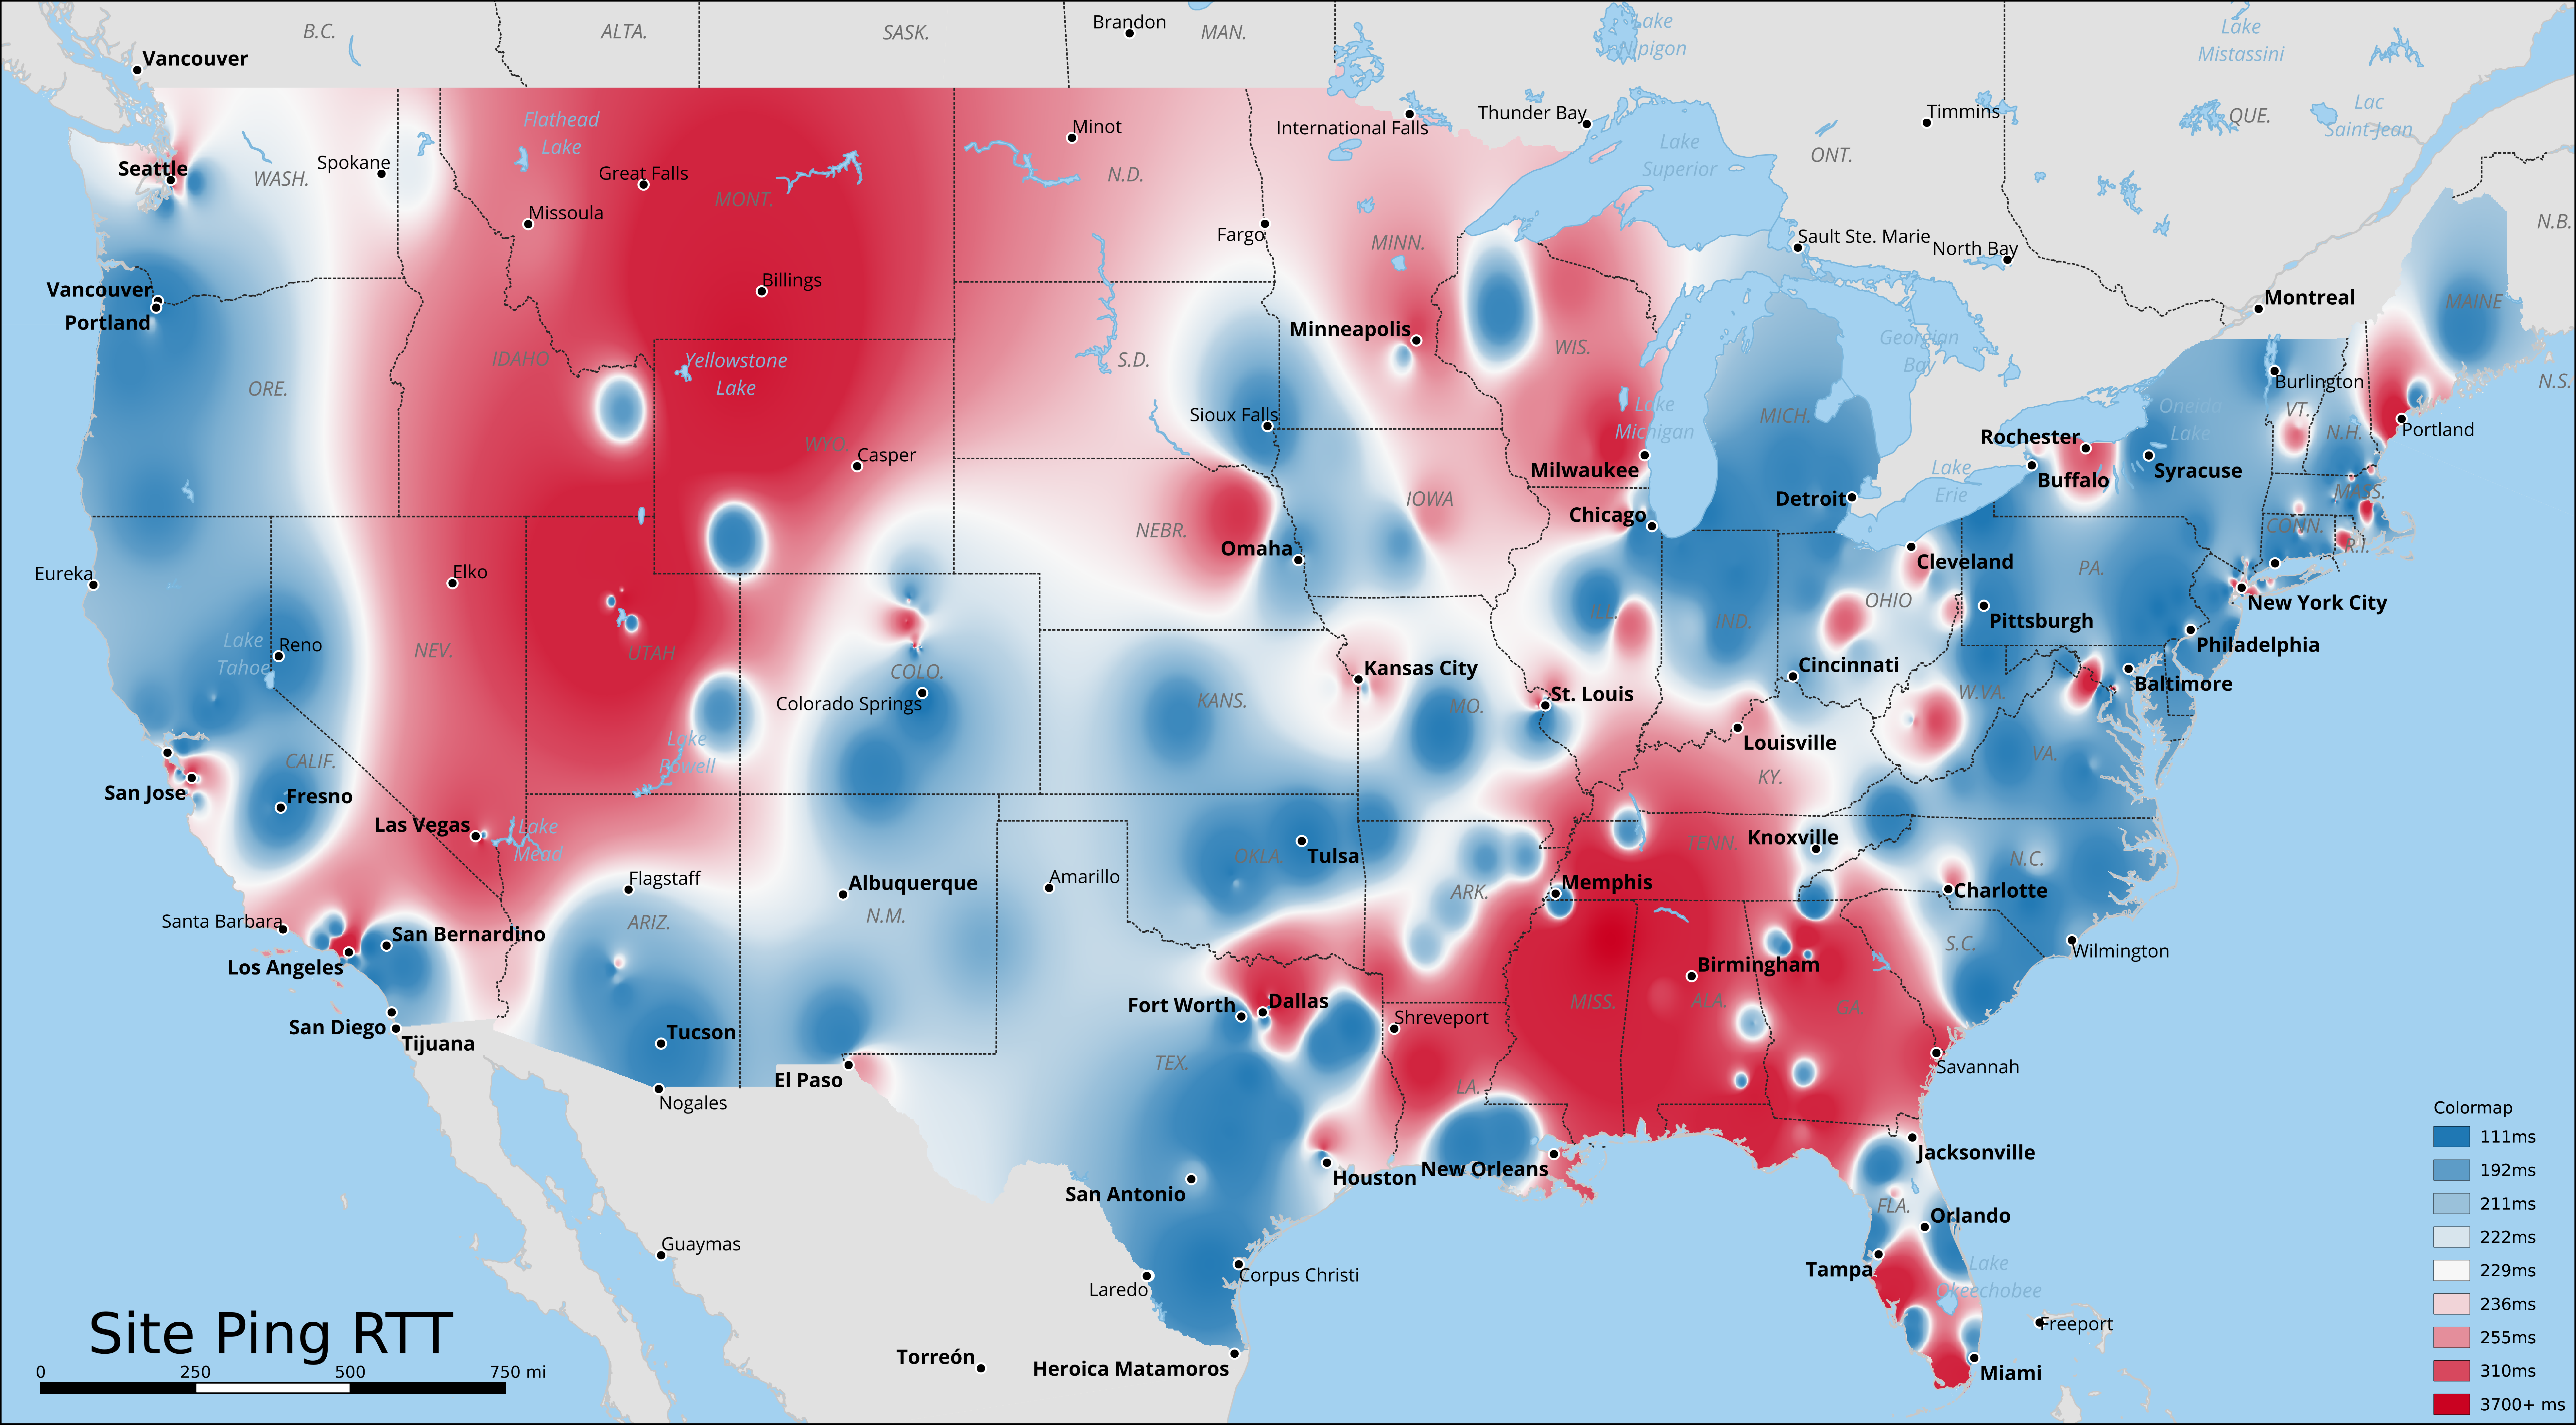
\includegraphics[width=0.85\textwidth]{images/siteping/site_ping_rtt_idw.jpg}
    \caption{Final Heat Map}
    \label{fig:siteping)_heatmap}
\end{figure}

    \section{Summary}

We drew up three different methods for collecting data that could be analyzed using different means and evaluated with respect to different metrics. We also discussed several data collection methods that we considered but ultimately did not pursue due in impracticality, impossibility at this time, or other factors.

Since they are used for analysis on data collected from all methods, we also discussed the statistical methods used to guage differences between the states and determine if the data supports comparisons between them at that level of aggregation. As part of these methods we presented several novel ideas for visualizing these comparisons and a way to possibly work around imperfect data when sorting.

    
    % \newpage
    \chapter{Intra-DNS Server RTT: DNS Cache Manipulation}\label{sec:dns}
    This chapter focuses on evaluating internet connectivity based on the "\rtt to Regional Locations" (\cref{sec:definition_rtt_regional}), with a focus on measuring \dns infrastructure connectivity as a proxy for overall connectivity. \dns is a crucial component of the internet. By measuring a region's ability to resolve domain names using servers in other regions, we can evaluate how well the first region is connected to the rest of the country. To accomplish this, we used a method called \dns cache manipulation and over 900 \dns servers spread across the United States and measured the \rtt between them. The following sections detail the design, implementation, and results of this method.
    \section{Design}\label{sec:dns_design}
The \dns cache manipulation method is largely derived from the method used in "The Internet Connected Project", the project preceding this one \cite{Fakult2019}. The method makes use of two sets of geographically diverse \dns servers: one list each of recursive and authoritative servers. The basic principle rests on the concept of making requests directly to each of the recursive servers that \textit{must} make their way to the authoritative ones and deducing the time between the two. As \dns includes no mechanism for reporting the time taken between two servers, \dns cache manipulation must rely on the \rtt from when the local request is dispatched to when an answer is received.

\subsection{Collection Stages}\label{sec:dns_design_collection_stages}

Collecting data via \dns cache manipulation takes six stages of processing: three for pre-processing and three to make the actual measurements. The preparatory stages, server confirmation, reliability checks, and geolocation, eliminate servers that are not appropriate to include in the study.

\begin{figure}[h]
    \centering
    \includegraphics[width=\textwidth]{dns/diagrams/dns_cache_manipulation_diagram.png}
    \caption{DNS cache manipulation stages}
    \label{fig:dns_cache_manipulation_stage_diagram}
\end{figure}

\autoref{fig:dns_cache_manipulation_stage_diagram} shows the three stages required for data collection: priming the \dns cache, measuring latency to the recursive \dns server, and measuring the lookup time. We will now discuss all five stages in more detail.

\subsubsection{Confirmation of Server Status and Type}\label{sec:dns_des_server_conf}
Prior to running any tests, two lists of candidate recursive and authoritative servers are fed into tools that confirm their status as usable servers. For recursive servers, this process confirms that they are indeed public recursive servers. For authoritative candidates, it verifies that the server provides an answer for the domain it is expected to.

\subsubsection{Testing Reliability}

\missingfigure{Diagram, CoV definition}

% \todo{A diagram or two would definitely help. Also CoV def.}
Before actually using any of the servers for testing, we tested their reliability -- i.e. how consistent their response times were under constant parameters. After making repeated requests to each server, that in theory should have similar response times, we filter servers based on the \cv for the measured response times. This eliminated any servers with high variation from the testing. For recursive servers, priming the cache (see below) and then making repeated requests for the primed value served as the repeated requests. For authoritative servers, this was accomplished by making repeated requests for a random subdomain that the servers are authorities for through the \wpi recursive \dns server. This server is close enough to the machine we ran the tests on that the lag was minimal. The justification for running the filtering prior to testing is that each server included in the test increased the time required to run the entire test suite exponentially, as each recursive server was paired with each authoritative server.

\subsubsection{IP Geolocation}
Just as in the other methods described in this report, \dns cache manipulation utilized IP geolocation provided by MaxMind to determine the location of the servers under test.

\subsubsection{Priming the DNS Cache} 
The first step of the actual testing involves priming the target recursive server's cache. Say the target recursive server's \ip address is \texttt{1.2.3.4} and the target authoritative server provides answers for \texttt{example.com}. By making a \dns query to \texttt{1.2.3.4} for \texttt{example.com}, we get the target \dns server to cache the answer to the query.

\subsubsection{Measuring Latency} 
After the target recursive server has cached the answer for the query for \texttt{example.com}, it will use that cached answer to respond to subsequent requests without making any iterative requests. We can then make another request, identical to the one in the priming stage, and time it. To get a latency measurement, we do this several times back to back and take the lowest value, which indicates the best possible latency between the machine the measurements are being taken on and the recursive server.

\subsubsection{Measuring the Total RTT} 
The final step in the process is to measure the \rtt between the local machine and the target authoritative server and subtract the latency to get the final result. To do this, we make a query to the recursive server for \texttt{random.example.com}, where \texttt{random} is a randomly generated sub-domain that is unlikely to actually exist on the targeted domain. This random sub-domain forces the recursive server to get an answer. Because it already knows the authoritative server for \texttt{example.com}, it can skip the process of querying the root and \texttt{.com} servers and make an immediate query to the server for \texttt{example.com}. We measure the time for this entire process and then subtract the previously measured latency, leaving only the time between the target recursive server and the target authoritative server, which is recorded.
    \section{Implementation}\label{sec:dns_impl} % TODO: More descriptive name?

This section details the implementation of the methodology designed in the \cref{sec:dns_design}. The implementation utilizes the command line utility \texttt{dig} to make \dns requests, Python to wrap around dig to make parsing its output easier, a bash script, and the \texttt{parallel} command line utility to enable parallel processing.

\subsection{Tools and Setup}

The entirety of the data collection for \dns cache manipulation took place on two \wpi servers: \texttt{ccc.wpi.edu} and \texttt{rambo.wpi.edu}.

At its core, this method used the \texttt{dig} utility for making \dns requests - this is the same tool used in the prior project \cite{Fakult2019}. The template command used for all stages of testing is shown in \cref{fig:dig_template_command}.

\begin{code}[h]
    \centering
    \begin{minted}{bash}
>dig [@<target server>] <target_domain> time=2 tries=1 +stats
    \end{minted}
    \caption{Template \texttt{dig} command}
    \label{fig:dig_template_command}
\end{code}

Notably, this command template does not include the \texttt{+noall} flag, unlike the prior project \cite{Fakult2019}. By omitting this flag in our version, we preserve the status and records actually produced by the recursive \dns server. \cref{fig:generic_dig_output} is an example of such output (modified slightly for formatting). This output includes the status flag \texttt{NXDOMAIN} which would be omitted with the \texttt{+notall} parameter. This status flag confirms that the random subdomain for a given domain does indeed not resolve to anything - this is important for the testing because if it did, the recursive server may have had a cache for that subdomain, invalidating the lookup time check. Additionally, this version of the command include the \texttt{ANSWER} and \texttt{AUTHORITY} sections (depending on the lookup) which aid in validating the type of server and the responses they give. These too would be left out with the \texttt{+noall} flag.

\begin{code}[H]
    \centering
    \begin{minted}{text}
>dig @8.8.8.8 doesnotexist.wpi.edu +time=2 +tries=1 +stats

; <<>> DiG 9.11.3-1ubuntu1.11-Ubuntu <<>> @8.8.8.8 
doesnotexist.wpi.edu +time=2 +tries=1 +stats
; (1 server found)
;; global options: +cmd
;; Got answer:
;; ->>HEADER<<- opcode: QUERY, status: NXDOMAIN, id: 31928
;; flags: qr rd ra; QUERY: 1, ANSWER: 0, AUTHORITY: 1, 
ADDITIONAL: 1

;; OPT PSEUDOSECTION:
; EDNS: version: 0, flags:; udp: 512
;; QUESTION SECTION:
;doesnotexist.wpi.edu.          IN      A

;; AUTHORITY SECTION:
wpi.edu.               1799    IN     SOA    adns1.wpi.edu.
netops.wpi.edu. 2010473291 3600 600 1209600 3600

;; Query time: 88 msec
;; SERVER: 8.8.8.8#53(8.8.8.8)
;; WHEN: Thu Feb 06 00:12:43 STD 2020
;; MSG SIZE  rcvd: 98
    \end{minted}
    \caption{Generic \texttt{dig} output}
    \label{fig:generic_dig_output}
\end{code}

Instead of running the \texttt{dig} tool directly via a bash script, we wrapped it in a Python script for ease of parsing. This allowed for easy, consistent usage across stages, which we also implemented using Python, as well as thorough testing to ensure expected behaviour. This utility itself utilized the \texttt{subprocess} module to make \texttt{dig} calls.

As mentioned, each stage in this method was implemented using Python, separating into several scripts. These were all brought together with a bash script and the \texttt{parallel} utility \cite{Tange2011}, which allowed for parallelization, greatly reducing the time required for testing.

\begin{code}[h]
    \centering
    \begin{minted}{bash}
>./parallel -a test_pairs.csv --colsep , --header '.*\n' 
    --progress --eta --jobs $JOB_COUNT 
    ./run_test.py {1} {2} {3} $TEST_TRY_COUNT $TIMEOUT 
    >> results/test_results.csv
    \end{minted}
    \caption{Sample \texttt{parallel} command}
    \label{fig:dns_sample_parallel_command}
\end{code}

\Cref{fig:dns_sample_parallel_command} shows the parallel command used to run the primary portion of the test. It uses a \csv listing the pairs of recursive and authoritative \dns servers and pipes them into the Python script \texttt{run\_test.py} before outputting the results. This is done with \texttt{JOBCOUNT} parallel jobs, which was configured to 32 jobs for each batch.

\subsection{Candidate DNS server lists}

Initial lists of both types of \dns servers were provided to us by our advisor, Professor Craig Wills. After performing initial verification of these servers, we augmented the list by searching through a list of `.gov` domains filtered by the states we needed to fill in gaps for. In total, these lists included 535 authoritative servers and 1225 recursive servers (prior to final filtering).

Note: the final list of recursive servers did not include any located in the state of Rhode Island despite an extensive search for one.

\subsection{Pre-processing Stages}

These stages ran prior to any actual data collection in an effort to streamline and shorten that collection processes. Each ran as one or more separate steps in the overall script, in the order presented.

\subsubsection{Confirmation of Server Status and Type}\label{sec:dns_impl_confirmation_of_status_and_type}

The code in \cref{fig:auth_conf_snippet} is what we used to confirm that an expected authoritative server was indeed an authoritative server. The request for the domain tied to the server was directed directly to the its \ip address. If there was a result (i.e. \texttt{dig} output a valid result), the status of that result was \texttt{NOERROR} (the server was able to generate a response for the given domain) and the \texttt{AUTHORITY} section of the response was non-zero in length, the server was confirmed as a authoritative for the expected domain.
\begin{code}[H]
\centering
    \begin{minted}{python}
result is not None 
    and result.status == "NOERROR" 
    and result.AUTHORITY > 0
    \end{minted}
    \caption{DNS Authoritative Confirmation Snippet}
    \label{fig:auth_conf_snippet}
\end{code}

The code use to confirm recursive servers, shown in \cref{fig:rec_conf_snippet}, was similar: there must be a result with an answer. However, it must also not have the phrase \texttt{Recursion requested but not available}. Additionally, it is allowed to have responses in the \texttt{ANSWER} section instead of just in the \texttt{AUTHORITY} section.

\begin{code}[H]
\centering
    \begin{minted}{python}
result is not None 
    and result.status == "NOERROR" 
    and not result.recursion_not_available 
    and (result.ANSWER > 0 or result.AUTHORITY > 0)
    \end{minted}
    \caption{DNS Recursive Confirmation Snippet}
    \label{fig:rec_conf_snippet}
\end{code}

\subsubsection{Testing Reliability}

\Cref{fig:auth_reliability_snippet} is a snippet of code, modified for formatting, that we used to verify the reliability of candidate authoritative servers. The code was passed a domain and \ip address for the authoritative server under tests. For a given number of trials, configured to 20 for every batch, the query time for a request made directly to the authoritative server for a domain we have already confirmed it was an authority for, was recorded (for a definition of a valid result, see \cref{sec:dns_impl_confirmation_of_status_and_type} and \cref{fig:auth_conf_snippet}). After all results were recorded, the authoritative server's \ip address was output if there were at least two successful results and the \cv was less than or equal to the threshold, configured to 0.5 for all tests.

\begin{code}[H]
\centering
    \begin{minted}{python}
    for _ in range(trials):
        result = run_dig(domain=domain, target_server=target_ip)
        if <result is valid>:
            results.append(result.query_time)
    if len(results) >= 2 and stdev(results)/mean(results) <= max_cov:
        print("{},{}".format(target_ip, generate_statistics(results)))
    \end{minted}
    \caption{Authoritative Server Reliability Snippet}
    \label{fig:auth_reliability_snippet}
\end{code}

Similarly, \cref{fig:rec_reliablility_snippet} shows a snippet for measuring the reliability of a candidate recursive server. A domain for testing (\texttt{cnn.com} for all runs) and a recursive server \ip address were passed in. First, the cache is primed to ensure the domain is cached in the server and then the query time for requesting that same domain from the server is recorded for a given number of trials (again, configured to 20 for each batch). Finally, if there were at least two results and the \cv met the threshold (0.5 for all testss), the domain was output as reliable. This is essentially making repeated latency measurements and ensuring that the results are consistent.

\begin{code}[H]
\centering
    \begin{minted}{python}
    run_dig(domain=domain, target_server=recursive_ip)
    for _ in range(trials):
        result = run_dig(domain=domain, target_server=recursive_ip)

        if <result is valid>:
            results.append(result.query_time)
    if len(results) >= 2 and stdev(results)/mean(results) <= max_cov:
        print("{},{}".format(recursive_ip, generate_statistics(results)))
    \end{minted}
    \caption{Recursive Server Reliability Snippet}
    \label{fig:rec_reliablility_snippet}
\end{code}

Note that both checks also output other statistics alongside the servers. These included the measurement mean, median, standard deviation, and variance. This gave us the option to do further analysis on server reliability, which we opted not to pursue.

\subsubsection{IP Geolocation}

To determine the physical location of the \dns servers, we used MaxMind, which provided coordinates and the server's state.

\subsection{Data Collection Stages}

These three stages are all contained within a single script and are run back-to-back-to-back with each other. The two main parameters for the script are a single \ip address, \texttt{recursive\_ip}, corresponding to a recursive server and a domain name, \texttt{authoritative\_domain}, and \ip address, \texttt{authoritative\_ip}, corresponding to the an authoritative server.

\subsubsection{Priming the DNS Cache}

Priming the \dns cache was performed by making a single \dns query to \texttt{recursive\_ip} for \texttt{authoritative\_domain}. This request did not include any randomized subdomain and occurred immediately prior to latency measurement.

\subsubsection{Measuring Latency}

\Cref{fig:dns_latency_snippet} shows the code that we used to measure the latency between the testing location and the recursive \dns server under test. For all tests, \texttt{tries = 10}, meaning that for each test for a given server pair, there were 10 latency measurements. Of the measurements, we kept the lowest one, as this indicated the shortest observed latency.

\begin{code}[H]
\centering
    \begin{minted}{python}
[run_dig(domain=authoritative_domain, 
        target_server=recursive_ip, 
        time=TIME_LIMIT) 
    for _ in range(tries)]
    \end{minted}
    \caption{DNS Latency Snippet}
    \label{fig:dns_latency_snippet}
\end{code}

The authoritative domain is provided without any subdomain, as we know that, due to the cache priming stage, the domain is cached in the recursive server.

\subsubsection{Measuring Lookup RTT}

Similar to the snippet for measuring latency, \cref{fig:dns_lookup_rtt_snippet} shows the snippet for measuring the total lookup time. Notably, a 12 character, randomized subdomain is added to the target authoritative server's domain. Once again, the number of observations was configured to 10 for all trials, and the minimum observed value was kept.

\begin{code}[H]
\centering
    \begin{minted}{python}
[run_dig(domain="{}.{}".format(rand_subdomain(), authoritative_domain),
        target_server=recursive_ip, 
        time=TIME_LIMIT) 
    for _ in range(tries)]
    \end{minted}
    \caption{DNS Lookup RTT Snippet}
    \label{fig:dns_lookup_rtt_snippet}
\end{code}

To calculate the final \rtt observed in a given test for a given pair of servers, we simply subtracted the lowest latency measurement from the lowest round-trip measurement to get the best possible \rtt between the recursive \dns server and the authoritative \dns server.
    \section{Collection Results}\label{sec:dns_results} % TODO Better section name?

Using the implementation outlined in the previous section, we ran four batches of data collection. This section provides an overview of the results of that collection, including issues we encountered and potential future mitigations for these issues.

\subsection{Server Reliability Filtering}

After filtering authoritative and recursive \dns servers for testing reliability (max coefficient of variation in repeated tests = 0.75), we were left with 387 authoritative servers across 50 states and the District of Columbia and 654 recursive servers across 49 states and the District of Columbia. We could not locate an open recursive \dns server, even unreliable, in the state of Rhode Island. \Cref{fig:dns_cache_manipulation_map_of_authoritative_servers} and \cref{fig:dns_cache_manipulation_map_of_recursive_servers} show the locations of the final server lists for authoritative servers and recursive servers respectively.

\begin{figure}[htb]
    \centering
    \includegraphics[width=0.75\textwidth]{images/dns/server_locations/auth_server_locations.png}
    \caption{Map of authoritative DNS servers}
    \label{fig:dns_cache_manipulation_map_of_authoritative_servers}
\end{figure}

\begin{figure}[htb]
    \centering
    \includegraphics[width=0.75\textwidth]{images/dns/server_locations/rec_server_locations.png}
    \caption{Map of recursive DNS servers}
    \label{fig:dns_cache_manipulation_map_of_recursive_servers}
\end{figure}

\subsection{Data Collection}

Data collection was done in two main batches, along with two supplemental ones to add additional servers and increase geographical coverage. All runs used \texttt{cnn.com} as the domain used to confirm candidate server's status as recursive servers and to test the recursive server's reliability.

\begin{table}[htb]
    \centering
    \begin{tabular}{p{1cm}||p{2cm}|p{2cm}|p{2cm}|p{2cm}|p{4cm} }
    %  \multicolumn{6}{c}{\textbf{Batch Overview}} \\
    %  \hline
     \textbf{\#} & \textbf{Trial Count} & \textbf{Timeout} & \textbf{Records} & \textbf{Runtime} & \textbf{Notes} \\
     \hline
     1 & 5 & 2s & 1,831,495 & 62h & \\
     2 & 10 & 3s & 3,763,311 & 244h & \\
     3 & 10 & 3s & 4,920 & 9m  & Sup. for VT rec. \\
     4 & 10 & 3s & 7,320 & 11m & Sup. for HI auth. \\
     \hline
     \multicolumn{3}{r|}{\textbf{Total}} & 5,607,046 & 306 hours & \\
    \end{tabular}
    \caption{Overview of DNS batch runs}
    \label{tab:dns_batch_overview}
\end{table}

Again, as \cref{tab:dns_batch_overview} shows, the vast majority of data was collected over the course of two collection runs, \#1 and \#2. The first run only conducted five trials for each authoritative-recursive server pair and limited the timeout to for each \texttt{dig} command to two seconds, whereas subsequent runs ran with ten trials and a three second timeout. There are two reasons for this. First, the initial batch was run on \texttt{ccc.wpi.edu}, which has more limitations than the machine used for subsequent runs, \texttt{rambo.wpi.edu}. Additionally, that run was the first major step up from the more limited development test runs and we wanted to minimize time lost in the event something went wrong. On subsequent tests, we had more confidence in the collection scripts and were able to let it run for longer unsupervised.

Batch \#3 was run with a limited number of recursive servers located only in Vermont (with the full authoritative server list) while batch \#4 ran with a limited number of authoritative servers located only in Hawaii (with the full recursive server list). These were run after we discovered that we lacked data of the given type for these states. 

We ran into one issue with batch \#4: the collection scripts randomize the order of all pairs under test to minimize the repetitive requests to the same \dns servers in too short of a time period. However, in both supplemental tests, there were only small numbers of recursive servers (for \#3) or authoritative servers (for \#4). In batch \#4, this resulted in repetitive requests to the same authoritative server in a short period of time, which in turn caused WPI's IT system to believe we were using a \dns tunnel. The use of such a tunnel is prohibited under WPI's Acceptable Use Policy and resulted in a temporary suspension of network privileges.

    \section{Analysis}\label{sec:dns_analysis}

With the data we collected, we conducted two major approaches at analysis. The first approach treated every measurement for a recursive server in a give state as equal and gave each state a score based on these measurements aggregated together. The second method first aggregated measurements within one state based on the authoritative state the measurement was made with, which also gave us the opportunity to weight connections to states differently.

\subsection{Distance Normalization}
One of the initial steps in processing the data collected involved adding an additional field for \rtt normalized by the distance between the points being connected. As mentioned earlier in this report, by normalizing for distance, we can form another measurement that allows for analysis of connectivity as related to the \textit{ideal} speed of connection, the speed of light.

Additionally, calculating the speed of the connection, not just the total \rtt, allowed us to filter out measurements that were faster than the speed of light. Such measurements were likely the result of anomalous latency readings, causing the calculated \rtt to be far lower than physically possible. In total, this initial filter eliminated 418,625 measurements (7.5\%) from the total dataset.

\subsection{Data Characterization}

\Cref{fig:dns_analytics_median_dist} shows the distribution of the median true \rtt values for all locations. It shows that the data takes on a bimodal distribution with peaks around 45ms and 68ms with a heavy bias towards the former.

\begin{figure}[htb]
    \centering
    \includegraphics[width=0.75\textwidth]{images/dns/dist_raw_data/dns_rtt_median_distribution.png}
    \caption{DNS RTT median distribution}
    \label{fig:dns_analytics_median_dist}
\end{figure}

\subsubsection{Normalized RTT}

After normalizing by distance, the bimodality all but disappears, as \cref{fig:dns_analytics_norm_median_dist} shows. In this chart, the distribution pears around 30km/ms.

\begin{figure}[htb]
    \centering
    \includegraphics[width=0.75\textwidth]{images/dns/dist_raw_data/dns_norm_rtt_median_distribution.png}
    \caption{DNS normalized RTT median distribution}
    \label{fig:dns_analytics_norm_median_dist}
\end{figure}

\subsection{Heat Maps}

\Cref{fig:dns_true_rtt_heatmap} shows a heatmap based on true \dns \rtt measurements. This map shows that a significant portion of Western US has poor \dns \rtts. In contrast to the West, a majority of the the East Coast performs better. As we discuss later, this is likely due to the higher quantity of authoritative servers present in the East. Another highlight is that the South is rather inconsistent: Mississippi is probably the most homogeneous in being bad, but Alabama, Georgia, Louisiana, Tennessee, Missouri, and even eastern Texas are rather "splotchy", for lack of a better term.

\begin{figure}[htb]
    \centering
    \includegraphics[width=0.75\textwidth]{images/dns/heatmaps/dns_rtt_idw.png}
    \caption{DNS true RTT heatmap}
    \label{fig:dns_true_rtt_heatmap}
\end{figure}

\Cref{fig:dns_normalized_rtt_heatmap} shows a similar heatmap, but for distance normalized \dns \rtt data. In stark contrast to the prior map, the West coast displays significantly better performance - likely due to the distance to eastern authoritative servers being cancelled out. The Midwest and mid-Atlantic regions fare much worse, while the South is far more consistent in its poor results. The two main regions that remain consistent between the two maps are the North East and Colorado/Wyoming.

\begin{figure}[htb]
    \centering
    \includegraphics[width=0.75\textwidth]{images/dns/heatmaps/dns_speed_of_light_idw.png}
    \caption{DNS normalized RTT heatmap}
    \label{fig:dns_normalized_rtt_heatmap}
\end{figure}

\subsection{Aggregation by Server Pairs}
Since there we multiple data points for each recursive-authoritative server pair, the first step in aggregating the data was to aggregate by these server pairs. To do this, we removed points within each pair that had a z-score greater than a given threshold \texttt{z} as these were considered outliers within their pairs. We then computed the \cv of each pair with the remaining values and discarded any pairs with a result greater than a given threshold \texttt{v} - these pairs did not have consistent measurements and were considered unreliable.

\begin{table}[htb]
    \centering
    \begin{tabular}{ l|l|l  }
      & \textbf{True \rtt records dropped} & \textbf{Normalized \rtt records dropped} \\
     \hline
      \texttt{z=3} & 92,553/5,188,421 (1.8\%) & 63,008/5,188,421 (1.2\%) \\
      \texttt{z=2} & 269,651/5,188,421 (5.2\%) & 237,353‬/5,188,421 (4.6\%) \\
      \texttt{z=1} & 1,362,184/5,188,421 (26.3\%) & 1,389,031‬/5,188,421 (26.8\%) \\
     \hline
    \end{tabular}
    \caption{DNS Z-score filtering}
    \label{tab:dns_z_filtering}
\end{table}

\begin{table}[htb]
    \centering
    \begin{tabular}{p{1.6cm}|p{4cm}|p{4cm}|p{4cm}}
         & \texttt{z=3} (\texttt{n=381,333}) & \texttt{z=2} (\texttt{n=381,333}) & \texttt{z=1} (\texttt{n=381,333}) \\
        \hline
        \texttt{v=0.05} & 193,099 (50.6\%)  & 167,618 (44.0\%) & ‭92,799 (24.3\%) \\
        \texttt{v=0.10} & 111,294 (29.2\%) & 92,023 (24.1\%) & 40,889 (10.7\%)‬\\
        \texttt{v=0.20} & 52,239 (13.7\%) &  40,353 (10.6\%) & 13,262 (3.5\%)\\
        \texttt{v=0.50} & 9,330 (2.4\%) &  6,333 (1.7\%) & 1,809 (0.5\%)\\
        \texttt{v=1.00} & 1,741 (0.5\%) &    766 (0.2\%) & 176 (\textapprox0.0\%) \\
        \hline
    \end{tabular}
    \caption{True RTT DNS pair CV filtering}
    \label{tab:dns_unnorm_cv_filtering}
\end{table}

\begin{table}[htb]
    \centering
    \begin{tabular}{p{1.6cm}|p{4cm}|p{4cm}|p{4cm}}
         & \texttt{z=3} (\texttt{n=382,963}) & \texttt{z=2} (\texttt{n=382,963}) & \texttt{z=1} (\texttt{n=382,963}) \\
        \hline
        \texttt{v=0.05} & 192,522 (50.3\%) & 166,514 (43.5\%) & 87,383 (22.8\%) \\
        \texttt{v=0.10} & 109,493 (28.6\%) & 89,906 (23.5\%) & 35,553 (9.3\%) \\
        \texttt{v=0.20} & 48,414 (12.6\%) & 37,623 (9.8\%) & 10,579 (2.8\%) \\
        \texttt{v=0.50} & 6,304 (1.6\%) & 4,570 (1.2\%) & 1,314 (0.3\%) \\
        \texttt{v=1.00} & 1,038 (0.3\%) &    415 (0.1\%) & 126 (\textapprox0.0\%) \\  
    \end{tabular}
    \caption{Normalized RTT DNS pair CV filtering}
    \label{tab:dns_norm_cv_filtering}
\end{table}

We chose to proceed with \texttt{v=1.0} and \texttt{z=2}, which left the vast majority of pairs in the data set excluding only the most inconsistent measurements. The reasoning behind this is that we aren't just interested in stable connections - so we left potentially unstable or inconsistent measurements in the data set.

\subsection{Aggregating Pairs by Recursive Server State}

One option to further aggregate the pair data is to group it by the location of the recursive server in each pair. This results in a list of \rtts, either true or normalized by distance, that can be aggregated into a single value for each state. This is one way of making comparisons between states.

\subsubsection{Initial State Rankings}

\Cref{tab:dns_only_recursive_initial_state_rankings} shows the results of ranking states by the median of each measurement in that state. There are two different rankings, one each for the true \rtt and the distance normalized \rtt, based on data filtered with \texttt{z=2} and \texttt{v=1.0}. As with all \dns data, there is no ranking for Rhode Island.

\todo{Units}
\begin{longtable}{lrr||lrr}
% \toprule
  \multicolumn{3}{c||}{True RTT} & \multicolumn{3}{c}{Normalized RTT} \\
     State &  Rank & Value &      State & Rank & Value \\
\midrule
\endhead
\midrule
\multicolumn{6}{r}{{Continued on next page}} \\
\midrule
\endfoot
% \bottomrule
\endlastfoot
        WY &    1 &  30.0 &             HI &    1 &  91.0 \\
        VA &    2 &  31.0 &             WY &    2 &  54.5 \\
        DC &    2 &  31.0 &             AK &    3 &  47.4 \\
        WV &    4 &  32.0 &             CA &    4 &  45.5 \\
        NY &    4 &  32.0 &             OR &    5 &  43.9 \\
        NJ &    6 &  33.0 &             NV &    6 &  43.7 \\
        MD &    7 &  34.0 &             CO &    7 &  43.6 \\
        SC &    8 &  34.5 &             NY &    8 &  43.0 \\
        CO &    9 &  38.0 &             UT &    9 &  42.7 \\
        NH &   10 &  38.5 &             ID &   10 &  42.0 \\
        IL &   11 &  39.0 &             WA &   11 &  41.8 \\
        MI &   12 &  40.0 &             NH &   12 &  41.7 \\
        PA &   12 &  40.0 &             AZ &   13 &  41.0 \\
        WI &   12 &  40.0 &             NJ &   14 &  40.9 \\
        NC &   15 &  41.0 &             MA &   15 &  40.7 \\
        TX &   16 &  42.0 &             VA &   16 &  37.1 \\
        MA &   16 &  42.0 &             FL &   17 &  37.0 \\
        OH &   16 &  42.0 &             TX &   18 &  36.8 \\
        IN &   19 &  43.0 &             MD &   19 &  36.4 \\
        GA &   19 &  43.0 &             DC &   20 &  35.8 \\
        MN &   21 &  45.0 &             SC &   21 &  34.6 \\
        OK &   22 &  46.0 &             CT &   22 &  33.6 \\
        MO &   22 &  46.0 &             PA &   23 &  33.3 \\
        LA &   22 &  46.0 &             NC &   24 &  32.4 \\
        AR &   22 &  46.0 &             MT &   25 &  32.0 \\
        CT &   22 &  46.0 &             VT &   26 &  31.6 \\
        FL &   27 &  47.0 &             MI &   27 &  31.5 \\
        IA &   28 &  48.0 &             WI &   28 &  30.6 \\
        KY &   29 &  49.0 &             WV &   29 &  30.6 \\
        NE &   30 &  49.5 &             NM &   30 &  30.4 \\
        UT &   31 &  50.0 &             MN &   31 &  30.0 \\
        VT &   32 &  51.0 &             ME &   32 &  29.8 \\
        TN &   33 &  52.0 &             GA &   33 &  29.6 \\
        AL &   34 &  53.0 &             ND &   34 &  29.4 \\
        AZ &   34 &  53.0 &             LA &   35 &  29.3 \\
        DE &   34 &  53.0 &             OK &   36 &  28.9 \\
        NV &   34 &  53.0 &             SD &   37 &  28.6 \\
        ID &   38 &  54.0 &             NE &   38 &  28.3 \\
        SD &   39 &  56.0 &             IL &   39 &  28.1 \\
        KS &   39 &  56.0 &             DE &   40 &  27.6 \\
        ND &   41 &  59.0 &             MO &   41 &  26.4 \\
        CA &   42 &  59.5 &             AR &   42 &  26.2 \\
        NM &   43 &  60.0 &             OH &   43 &  25.4 \\
        HI &   43 &  60.0 &             IA &   44 &  25.0 \\
        MS &   45 &  62.0 &             AL &   45 &  24.5 \\
        OR &   46 &  65.0 &             IN &   46 &  24.4 \\
        WA &   47 &  67.0 &             KS &   47 &  22.9 \\
        ME &   48 &  67.5 &             KY &   48 &  21.9 \\
        MT &   49 &  71.0 &             TN &   49 &  21.6 \\
        AK &   50 &  99.2 &             MS &   50 &  20.4 \\
        RI &   -- &    -- &             RI &   -- &    -- \\
        \caption{Initial State Rankings -- Recursive Location Aggregation}
        \label{tab:dns_only_recursive_initial_state_rankings}
\end{longtable}


Notably, \cref{tab:dns_only_recursive_initial_state_rankings} indicates that Wyoming ranks in the top five for both rankings. No other state appears performs so consistently well. Additionally, the rankings show that while Hawaii and Alaska rank near or at the bottom for true \rtt, both states appear near the top of the normalized ranking. This shows that while the some states, Alaska and Hawaii in particular, may be inherently unconnected from the rest of the United States, the quality of their connection could be relatively high and merely dominated by sheer distances.

\subsubsection{Evaluating State Rankings}

To determine the validity of the rankings proposed above we used the Kruskal-Wallis test to determine whether there was evidence that datasets for different states came from different distributions. If we cannot reject the null hypothesis that they are from the same distribution, we cannot rank them in distinct positions. After running Kurskals between the datasets for each of the 49 states and DC, we used a p value threshold of 0.05 to determine if we could differentiate two states from each other. 

% \begin{figure}[h]
\begin{wrapfigure}[28]{L}{0.65\textwidth}
    \centering
    \includesvg[width=0.65\textwidth]{images/dns/analysis_no_auth_agg/rtt/no_auth_agg_true_rtt_graph.svg}
    \caption{DNS true RTT indistinguishability graph}
    \label{fig:dns_true_rtt_indistinguishable_states_graph}
\end{wrapfigure}
% \end{figure}

For true \rtt, \cref{fig:dns_true_rtt_indistinguishable_states_graph} shows a graph with a node for each of the 49 states and DC and a link between each pair of nodes where the Kruskal-Wallis test between the two yielded a p value greater than 0.05, indicating that there is no evidence of a difference between the two states. Each the y-position for each state in the graph is dictated by its ranking in the the initial ranking table (ties were broken up arbitrarily for readability and the x-position is arbitrary). 

Note that the top seven states in the true \rtt ranking in \cref{tab:dns_only_recursive_initial_state_rankings}, WY, VA, DC, WV, NY, NJ, and MD, form a distinct sub graph. Similarly, the states ranked \#9-12, IL, CO, NH, and MI, form another distinct sub graph. This indicates that while the states that make up these two groups cannot be distinguished from one another (i.e. there is no evidence that Wyoming is better than Virginia), we can state the the entirety of the first group is better than the entirety of the second group.

Similar to the groups at the top of the ranking, there are distinct groups at the bottom. Kruskals identified Alaska, \#50, as entirely different. However, the six preceding states ranked \#43(t) to \#49, HI, MS, OR, WA, ME, and MT, are a distinct sub graph, as are the three states preceding them, ND, NM, and HI. Note that in the initial ranking, New Mexico and Hawaii are tied for \#43, but are identified as distinct using Kruskals.

Also notable is Louisiana: the state ranks \#22(t), but is labeled as indistinguishable from Arizona, \#34(t), and Nevada, \#34(t).

\begin{figure}[htb]
    \centering
    \includegraphics[width=0.75\textwidth]{images/dns/analysis_no_auth_agg/rtt/no_auth_distinct_rtt_map.png}
    \caption{DNS true RTT state groupings}
    \label{fig:dns_true_rtt_indistinguishable_states_map}
\end{figure}

\Cref{fig:dns_true_rtt_indistinguishable_states_map} maps the each distinct sub graph to a separate color (graphs are numbered by in the order of their highest ranked consituent state). This highlights some patterns and some oddities. For example, seven of the top eight states, represented by groups 1 and 2, are located on the East Coast, with Wyoming being the odd state out. The Midwest and the western Mountain region are dominated by states in groups 7 and 8. The Great Lakes region consists primarily of states in groups 3 and four. The West Coast and Hawaii did not fair as well as the East Coast with California, Oregon, and Washington (and Hawaii) in groups 9 and 10. Meanwhile, the South is a bit of a "hodge-podge" of groups, indicating a lack of consistency there.

\begin{figure}[htb]
    \centering
    \includegraphics[width=0.75\textwidth]{images/dns/analysis_no_auth_agg/rtt/no_auth_agg_rtt_confidence.png}
    \caption{DNS true RTT confidence intervals}
    \label{fig:dns_true_rtt_confidence_intervals}
\end{figure}

Finally, for true \rtt, \cref{fig:dns_true_rtt_confidence_intervals} shows bootstrapped confidence intervals for each state. With a few exceptions, bounds are fairly tight, indicating high confidence that the ranking listed in \cref{tab:dns_only_recursive_initial_state_rankings} is reliable. One of the notable exceptions is Wyoming, which has a much higher confidence interval than its neighbors in the "good" \rtt region. One possible cause for this may be the fact that Wyoming only had one recursive server in it. However, this was also the case for other servers that did not exhibit the behavior that Wyoming did.

Similar to the graph for true \rtt, \cref{fig:dns_normalized_rtt_indistinguishable_states_graph} is a graph of states in the normalized \rtt ranking that are indistinguishable. This graph includes a much larger and messier middle group consisting of 27 states. Hawaii, ranked \#1 is an independent node, as is California at \#4, with Alaska and Wyoming forming a pair between these two. At the bottom, Mississippi is distinctly alone. The second largest distinct subgroup consists of 10 states spanning from \#5 to \#15, with Utah distinct from all of them, but ranked \#9.

% \begin{figure}[htb]
\begin{wrapfigure}[27]{R}{0.50\textwidth}
    \centering
    \includesvg[width=0.50\textwidth]{images/dns/analysis_no_auth_agg/rtt_normalized/no_auth_agg_norm_rtt_graph.svg}
    \caption{DNS normalized RTT indistinguishable states graph}
    \label{fig:dns_normalized_rtt_indistinguishable_states_graph}
\end{wrapfigure}
% \end{figure}

Overall, \cref{fig:dns_normalized_rtt_indistinguishable_states_graph} shows that while there are more completely distinct states in the normalized rankings, the states in the middle of the pack are dominated by a single large cluster.

Mapping the distinct sub graphs for normalized \dns \rtt shows a majority of the large, mid ranking sub graph is on the East Coast and in the Midwest, with some states in the Mountain region. The West Coast is comprised entirely of states in groups 3 and 4, which also contain some states in the North East.

\begin{figure}[htb]
    \centering
    \includegraphics[width=0.75\textwidth]{images/dns/analysis_no_auth_agg/rtt_normalized/no_auth_distinct_norm_rtt_map.png}
    \caption{Normalized RTT indistinguishability graph}
    \label{fig:dns_normalized_rtt_indistinguishable_states_map}
\end{figure}

\subsection{Aggregation by Authoritative State then Recursive State}

One shortcoming of aggregating pairs directly by the location of the recursive server is that this inherently weights the data by the number of authoritative servers in a single state. To compensate, this analysis approach first groups and aggregates by recursive server and authoritative server location. 

Given the presence of authoritative servers in every state, this creates a list of 51 measurements for each state with a recursive server. For example, all measurements between a recursive server in California and an authoritative server in Massachusetts are aggregated into a single measurement (using median) for California. This is then done for every other state with measurements from California, giving California a 51 measurement dataset, and then repeated for each state with a recursive server. 

To get a final value for a given state, each of these 51 measurements is averaged. Back to the example of California, this gives each state with measurements from California an equal weight in the final value for California. 

However, prior to averaging the 51 measurements for each state, we had the option of applying weights to the values. Again with the California example, we could apply a weight to the aggregated measurement between it and Massachusetts based on Massachusetts' population, \gdp, or other metric. For example, Massachusetts has a high population than Wyoming, so with a population based weighting scheme, the measurement to Massachusetts is valued higher than the measurement to Wyoming.

We chose to proceed with unweighted and population weighted aggregations. Weighting by population gives higher value to connections with states that have greater populations. Essentially, this creates a proxy for how well connected people in one state are to all other people in the United States.

\subsubsection{State Rankings}

\Cref{tab:dns_auth_initial_state_rankings} shows rankings based on this aggregation method, unweighted and population weighted, for both true \dns \rtt and normalized \dns \rtt. There are some shared patterns with the previous aggregation rankings: Wyoming ranks highly in all four, Alaska and Hawaii are at the bottom in both true \rtt metrics but rise to top when looking at the normalized rankings. Under true \rtt, all weighted \rtt values are lower than the values at the same rank in the unweighted column. This indicates states with higher populations have generally lower values than their counterparts, driving down the weighted metrics.

\begin{longtable}{lrr|lrr||lrr|lrr}
  \multicolumn{6}{c||}{\textbf{True RTT}} & \multicolumn{6}{c}{\textbf{Normalized RTT}} \\
\multicolumn{3}{c|}{\textbf{Unweighted}} & \multicolumn{3}{c||}{\textbf{Pop. Weighted}} & \multicolumn{3}{c|}{\textbf{Unweighted}} & \multicolumn{3}{c||}{\textbf{Pop. Weighted}} \\
     \textbf{State} & \textbf{Rank} & \textbf{(ms)} & \textbf{State} & \textbf{Rank} & \textbf{(ms)} &\textbf{State} & \textbf{Rank} & \textbf{(ms)} &\textbf{State} & \textbf{Rank} & \textbf{(ms)} \\
\midrule
\endhead
\midrule
\multicolumn{12}{r}{{Continued on next page}} \\
\midrule
\endfoot
\bottomrule
\endlastfoot
        VA &    1 &   39.1 &            WY &    1 &  35.7 &             HI &    1 &  104.5 &            HI &    1 &  106.5 \\
        NY &    2 &   39.2 &            VA &    2 &  37.0 &             WY &    2 &   77.3 &            WY &    2 &   80.1 \\
        WY &    3 &   39.5 &            NY &    3 &  37.2 &             AK &    3 &   46.4 &            AK &    3 &   48.9 \\
        NJ &    4 &   40.0 &            MD &    4 &  37.6 &             CA &    4 &   45.8 &            ID &    4 &   43.7 \\
        WV &    5 &   40.3 &            SC &    5 &  37.7 &             NV &    5 &   45.0 &            CO &    5 &   43.3 \\
        DC &    5 &   40.3 &            DC &    6 &  37.9 &             ID &    6 &   44.3 &            UT &    6 &   43.0 \\
        MD &    7 &   40.7 &            NJ &    7 &  38.5 &             UT &    6 &   44.3 &            CA &    7 &   42.0 \\
        CO &    8 &   41.5 &            WV &    8 &  38.9 &             AZ &    8 &   44.2 &            OR &    8 &   41.8 \\
        SC &    9 &   42.0 &            CO &    9 &  40.0 &             OR &    9 &   43.2 &            NY &    9 &   41.6 \\
        MI &   10 &   43.4 &            IL &   10 &  41.5 &             CO &   10 &   41.7 &            NV &    9 &   41.6 \\
        IL &   11 &   43.7 &            WI &   11 &  42.3 &             NY &   11 &   41.1 &            WA &   11 &   40.6 \\
        WI &   12 &   44.5 &            MI &   12 &  42.4 &             WA &   12 &   41.0 &            NH &   12 &   40.4 \\
        PA &   13 &   45.4 &            NC &   12 &  42.4 &             DC &   13 &   39.1 &            NJ &   13 &   39.1 \\
        NH &   14 &   45.9 &            TX &   14 &  43.1 &             NJ &   14 &   38.8 &            AZ &   13 &   39.1 \\
        NC &   14 &   45.9 &            PA &   15 &  43.2 &             VA &   15 &   38.0 &            MA &   15 &   37.9 \\
        TX &   16 &   46.9 &            NH &   16 &  43.9 &             NH &   16 &   37.8 &            MD &   16 &   37.7 \\
        OH &   17 &   47.0 &            OH &   17 &  45.1 &             FL &   17 &   37.7 &            DC &   17 &   37.6 \\
        UT &   18 &   48.0 &            GA &   18 &  45.9 &             TX &   18 &   37.6 &            VA &   18 &   37.0 \\
        MN &   19 &   48.1 &            MA &   19 &  46.1 &             MD &   19 &   37.5 &            TX &   19 &   36.8 \\
        IN &   20 &   48.3 &            MN &   20 &  46.3 &             SC &   20 &   36.3 &            FL &   20 &   36.3 \\
        MA &   21 &   48.4 &            IN &   20 &  46.3 &             MA &   21 &   35.9 &            CT &   21 &   36.2 \\
        AR &   22 &   49.9 &            OK &   22 &  46.6 &             CT &   22 &   34.4 &            SC &   21 &   36.2 \\
        GA &   23 &   50.1 &            AR &   23 &  46.9 &             WV &   23 &   33.6 &            WV &   23 &   32.9 \\
        OK &   24 &   50.6 &            UT &   24 &  47.9 &             NC &   24 &   33.0 &            PA &   23 &   32.9 \\
        MO &   25 &   51.0 &            LA &   24 &  47.9 &             PA &   25 &   32.2 &            VT &   25 &   32.8 \\
        LA &   26 &   52.3 &            CT &   26 &  48.7 &             VT &   26 &   31.9 &            NC &   26 &   32.7 \\
        CT &   27 &   52.7 &            MO &   26 &  48.7 &             LA &   27 &   31.6 &            MN &   26 &   32.7 \\
        IA &   28 &   53.2 &            FL &   28 &  49.1 &             MI &   28 &   31.5 &            MI &   28 &   32.2 \\
        NE &   29 &   53.5 &            IA &   29 &  51.1 &             NM &   29 &   30.9 &            WI &   29 &   31.8 \\
        VT &   30 &   53.6 &            NE &   30 &  51.2 &             GA &   30 &   30.8 &            LA &   30 &   30.8 \\
        FL &   31 &   53.7 &            VT &   31 &  52.6 &             MN &   31 &   29.8 &            NM &   30 &   30.8 \\
        ID &   32 &   54.0 &            NV &   32 &  52.9 &             WI &   31 &   29.8 &            MT &   32 &   30.6 \\
        AZ &   33 &   54.3 &            KY &   33 &  53.2 &             OK &   33 &   29.7 &            OK &   33 &   30.5 \\
        NV &   34 &   55.4 &            AZ &   34 &  53.4 &             IL &   34 &   29.2 &            IL &   34 &   30.1 \\
        KY &   35 &   56.0 &            ID &   35 &  53.7 &             MT &   35 &   29.0 &            NE &   35 &   29.8 \\
        SD &   36 &   58.7 &            TN &   36 &  54.7 &             AR &   36 &   28.1 &            GA &   35 &   29.8 \\
        TN &   37 &   59.3 &            AL &   37 &  56.2 &             NE &   37 &   27.9 &            SD &   37 &   29.6 \\
        CA &   38 &   60.1 &            CA &   38 &  56.9 &             SD &   38 &   27.7 &            ND &   38 &   29.5 \\
        AL &   39 &   60.7 &            DE &   39 &  57.1 &             ME &   38 &   27.7 &            ME &   39 &   29.4 \\
        NM &   40 &   60.9 &            KS &   40 &  57.9 &             OH &   40 &   27.1 &            AR &   40 &   28.2 \\
        DE &   41 &   61.4 &            SD &   41 &  58.3 &             ND &   41 &   26.4 &            OH &   41 &   27.4 \\
        KS &   42 &   61.8 &            NM &   42 &  58.8 &             MO &   41 &   26.4 &            DE &   42 &   27.3 \\
        OR &   43 &   63.2 &            ND &   43 &  61.7 &             AL &   43 &   26.0 &            MO &   43 &   27.2 \\
        ND &   44 &   64.6 &            OR &   44 &  63.4 &             IN &   44 &   25.7 &            IN &   44 &   26.4 \\
        WA &   45 &   67.3 &            MS &   45 &  63.9 &             DE &   45 &   25.4 &            IA &   45 &   26.2 \\
        MS &   46 &   67.4 &            HI &   46 &  65.3 &             IA &   46 &   24.8 &            AL &   46 &   25.2 \\
        HI &   47 &   69.7 &            WA &   47 &  66.8 &             KY &   47 &   23.1 &            KS &   47 &   24.1 \\
        MT &   48 &   71.9 &            MT &   48 &  70.7 &             MS &   48 &   22.9 &            KY &   48 &   23.4 \\
        ME &   49 &   77.6 &            ME &   49 &  75.5 &             TN &   49 &   22.4 &            TN &   49 &   23.0 \\
        AK &   50 &  100.4 &            AK &   50 &  99.1 &             KS &   49 &   22.4 &            MS &   50 &   22.0 \\
        RI &   -- &     -- &            RI &   -- &    -- &             RI &   -- &     -- &            RI &   -- &     -- \\
        
        \caption{Initial State Rankings -- Authoritative Location Aggregation}
        \label{tab:dns_auth_initial_state_rankings}
\end{longtable}

\subsubsection{Evaluating State Rankings}

As with the previous aggregation method, we began evaluating this approach by using the Kruskal-Wallis test. States were compared against each other using the 51 measurement dataset created by aggregating by the location of authoritative servers.

\Cref{fig:dns_auth_agg_s2s_true_rtt_graphs} shows the results of this analysis for true \rtt, with the unweighted results on the left and the population weighted results on the right. \Cref{fig:dns_auth_agg_s2s_norm_rtt_graphs} does the same for the normalized data. All four show roughly the same thing: with this analysis method, there are very few completely distinct states (Hawaii in the normalized data and Alaska in the unweighted true \rtt data). Overall, the unweighted data for both true \rtt and normalized \rtt show lower inter-connectivity, indicating that states are more distinguishable from each other when the data is not weighted.

\begin{figure}[htb]
    \centering
    \includesvg[width=0.45\textwidth]{images/dns/analysis_auth_agg/rtt/unweighted/analysis_auth_agg_graph_rtt_un.svg}
    \includesvg[width=0.45\textwidth]{images/dns/analysis_auth_agg/rtt/population/analysis_auth_agg_graph_rtt_pop.svg}
    \caption{Unweighted and population weighted rank graphs (true RTT)}
    \label{fig:dns_auth_agg_s2s_true_rtt_graphs}
\end{figure}

\begin{figure}[h]
    \centering
    \includesvg[width=0.45\textwidth]{images/dns/analysis_auth_agg/rtt_normalized/unweighted/analysis_auth_agg_graph_norm_rtt_un.svg}
    \includesvg[width=0.45\textwidth]{images/dns/analysis_auth_agg/rtt_normalized/population/analysis_auth_agg_graph_norm_rtt_pop.svg}
    \caption{Unweighted and population weighted graphs (normalized RTT)}
    \label{fig:dns_auth_agg_s2s_norm_rtt_graphs}
\end{figure}

In short, these graphs show that the rankings provided in \cref{tab:dns_auth_initial_state_rankings} are likely highly unreliable.

As a result, we continued by determining how many states each state is distinctly better than for each ranking. For example, if California is ranked above Wyoming and the p-value comparing the two is less than or equal to 0.05, California is considered to be distinctly better than Wyoming. On the other hand, if California is also ranked above Massachusetts but the p-value between the two is greater than 0.05, California does not gain credit for being distinctly higher than Massachusetts. States initially ranked above California would not be considered. \Cref{tab:dns_auth_agg_better_than} shows the results of this analysis.

\begin{longtable}{lrr|lrr||lrr|lrr}
\toprule
  \multicolumn{6}{c||}{True RTT} & \multicolumn{6}{c}{Normalized RTT} \\
\multicolumn{3}{c|}{Unweighted} & \multicolumn{3}{c||}{Pop. Weighted} & \multicolumn{3}{c|}{Unweighted} & \multicolumn{3}{c}{Pop. Weighted} \\
     State & Rank & Cnt. &         State & Rank & Cnt. &          State & Rank & Cnt. &         State & Rank & Cnt. \\
\midrule
\endhead
\midrule
\multicolumn{12}{r}{{Continued on next page}} \\
\midrule
\endfoot

\bottomrule
\endlastfoot
        VA &    1 &            40 &            WY &    1 &            24 &             HI &    1 &            49 &            HI &    1 &            49 \\
        WY &    2 &            39 &            NY &    1 &            24 &             AK &    2 &            42 &            AK &    2 &            28 \\
        NY &    3 &            36 &            VA &    3 &            23 &             CA &    3 &            38 &            WY &    3 &            20 \\
        WV &    3 &            36 &            DC &    3 &            23 &             ID &    3 &            38 &            CA &    4 &            18 \\
        DC &    3 &            36 &            MD &    5 &            21 &             NV &    5 &            36 &            NV &    5 &            15 \\
        NJ &    6 &            35 &            NJ &    6 &            18 &             UT &    5 &            36 &            OR &    6 &            12 \\
        MD &    6 &            35 &            WV &    7 &            16 &             OR &    7 &            31 &            UT &    7 &            11 \\
        SC &    8 &            34 &            SC &    8 &            13 &             WY &    8 &            30 &            ID &    8 &            10 \\
        CO &    9 &            32 &            MI &    9 &             9 &             AZ &    9 &            28 &            WA &    8 &            10 \\
        MI &    9 &            32 &            CO &   10 &             8 &             CO &    9 &            28 &            AZ &    8 &            10 \\
        IL &   11 &            31 &            IL &   10 &             8 &             NY &    9 &            28 &            CO &   11 &             9 \\
        WI &   12 &            30 &            WI &   12 &             7 &             WA &    9 &            28 &            NY &   11 &             9 \\
        PA &   13 &            28 &            NH &   12 &             7 &             TX &   13 &            26 &            FL &   11 &             9 \\
        NC &   13 &            28 &            PA &   14 &             6 &             FL &   13 &            26 &            TX &   11 &             9 \\
        NH &   15 &            26 &            NC &   14 &             6 &             NH &   13 &            26 &            DC &   15 &             8 \\
        OH &   16 &            23 &            OH &   16 &             5 &             NJ &   16 &            25 &            VA &   16 &             7 \\
        TX &   17 &            22 &            TX &   17 &             4 &             DC &   17 &            24 &            NH &   16 &             7 \\
        MN &   18 &            21 &            GA &   18 &             3 &             MD &   18 &            22 &            NJ &   18 &             6 \\
        IN &   18 &            21 &            MA &   18 &             3 &             MA &   18 &            22 &            MD &   18 &             6 \\
        MA &   20 &            20 &            MN &   18 &             3 &             VA &   18 &            22 &            MA &   20 &             4 \\
        GA &   20 &            20 &            IN &   18 &             3 &             SC &   21 &            20 &            SC &   20 &             4 \\
        UT &   22 &            19 &            FL &   22 &             2 &             NC &   22 &            12 &            MI &   22 &             1 \\
        AR &   22 &            19 &            VT &   22 &             2 &             CT &   23 &            11 &            NC &   22 &             1 \\
        OK &   24 &            18 &            IA &   22 &             2 &             MI &   23 &            11 &            WV &   22 &             1 \\
        MO &   25 &            17 &            MO &   22 &             2 &             LA &   23 &            11 &            KS &   25 &             0 \\
        LA &   26 &            15 &            LA &   22 &             2 &             PA &   26 &            10 &            AL &   25 &             0 \\
        CT &   26 &            15 &            UT &   22 &             2 &             WV &   27 &             9 &            KY &   25 &             0 \\
        FL &   26 &            15 &            AR &   22 &             2 &             GA &   28 &             7 &            IA &   25 &             0 \\
        IA &   29 &            14 &            OK &   22 &             2 &             NM &   29 &             6 &            ND &   25 &             0 \\
        NE &   29 &            14 &            CT &   22 &             2 &             MN &   29 &             6 &            IN &   25 &             0 \\
        VT &   31 &            12 &            CA &   31 &             1 &             WI &   29 &             6 &            MO &   25 &             0 \\
        ID &   31 &            12 &            OR &   31 &             1 &             MT &   32 &             5 &            DE &   25 &             0 \\
        KY &   31 &            12 &            ND &   31 &             1 &             OK &   32 &             5 &            OH &   25 &             0 \\
        AZ &   34 &            10 &            NM &   31 &             1 &             VT &   32 &             5 &            AR &   25 &             0 \\
        TN &   35 &             9 &            SD &   31 &             1 &             ND &   35 &             4 &            ME &   25 &             0 \\
        NV &   36 &             8 &            KS &   31 &             1 &             ME &   35 &             4 &            SD &   25 &             0 \\
        SD &   36 &             8 &            DE &   31 &             1 &             SD &   35 &             4 &            VT &   25 &             0 \\
        AL &   36 &             8 &            TN &   31 &             1 &             AR &   35 &             4 &            NE &   25 &             0 \\
        KS &   39 &             6 &            ID &   31 &             1 &             IL &   35 &             4 &            IL &   25 &             0 \\
        DE &   39 &             6 &            AZ &   31 &             1 &             NE &   40 &             3 &            OK &   25 &             0 \\
        NM &   41 &             5 &            KY &   31 &             1 &             MO &   41 &             1 &            MT &   25 &             0 \\
        CA &   42 &             4 &            NV &   31 &             1 &             KY &   42 &             0 &            NM &   25 &             0 \\
        ND &   43 &             3 &            NE &   31 &             1 &             MS &   42 &             0 &            LA &   25 &             0 \\
        MS &   43 &             3 &            AL &   31 &             1 &             IA &   42 &             0 &            WI &   25 &             0 \\
        OR &   45 &             2 &            MT &   45 &             0 &             TN &   42 &             0 &            MN &   25 &             0 \\
        WA &   46 &             1 &            WA &   45 &             0 &             IN &   42 &             0 &            TN &   25 &             0 \\
        HI &   46 &             1 &            ME &   45 &             0 &             AL &   42 &             0 &            PA &   25 &             0 \\
        MT &   46 &             1 &            MS &   45 &             0 &             OH &   42 &             0 &            CT &   25 &             0 \\
        ME &   46 &             1 &            HI &   45 &             0 &             DE &   42 &             0 &            GA &   25 &             0 \\
        AK &   50 &             0 &            AK &   45 &             0 &             KS &   42 &             0 &            MS &   25 &             0 \\
        RI &   -- &            -- &            RI &   -- &            -- &             RI &   -- &            -- &            RI &   -- &            -- \\


        \caption{DNS Authoritative Aggregation - Number of States Better Than}
        \label{tab:dns_auth_agg_better_than}
\end{longtable}


Perhaps most notable is that for the normalized \rtt data weighted by population, over half of states were not distinctly better than a single other state. Overall, the unweighted methodologies fared better at distinguishing states at the top and bottom. 

And again, Wyoming ranked highly in all tables - its worst rank is \#8 for unweighted normalized \rtt. Alaska and Hawaii rank low in the true \rtt metrics but are at the top for normalized.

\Cref{fig:dns_auth_agg_num_better_map_rtt} and \cref{fig:dns_auth_agg_num_better_map_norm_rtt}, show maps of the results in \cref{tab:dns_auth_agg_better_than}, where states with darker green coloring are distinctly better than more states than states that are colored grey. In \cref{fig:dns_auth_agg_num_better_map_rtt}, which show the true \rtt unweighted and weighted maps, East Coast states, and to a lesser degree Midwestern states, perform prominently better, with Colorado and Wyoming as the primary exceptions. When weights are applied, the only states that remain clearly above the rest are a handful of East Coast states and Wyoming.

\begin{figure}[htb]
    \centering
    \includegraphics[width=.6\textwidth]{images/dns/analysis_auth_agg/rtt/unweighted/num_better_than_map_rtt_un.png}\\
    \includegraphics[width=.6\textwidth]{images/dns/analysis_auth_agg/rtt/population/num_better_than_map_rtt_pop.png}
    \caption{DNS true RTT unweighted and population weighted ``better than'' map}
    \label{fig:dns_auth_agg_num_better_map_rtt}
\end{figure}

On the other hand, the normalized maps, \cref{fig:dns_auth_agg_num_better_map_norm_rtt} show Western states performing far better than the rest of the country, although some on the East Coast do fairly well. However, much of that performance is lost when weighted by population, where Western states are far more muted. One possible explanation for this is that while the normalized metric removes the distance barrier for the West, these states are also a great distance from the denser East Coast.

\begin{figure}[htb]
    \centering
    \includegraphics[width=0.6\textwidth]{images/dns/analysis_auth_agg/rtt_normalized/unweighted/num_better_than_map_norm_rtt_un.png}\\
    \includegraphics[width=0.6\textwidth]{images/dns/analysis_auth_agg/rtt_normalized/population/num_better_than_map_norm_rtt_pop.png}
    \caption{DNS normalized RTT unweighted  and population weighted ``better than'' map}
    \label{fig:dns_auth_agg_num_better_map_norm_rtt}
\end{figure}

Overall, these maps show that there are few meaningful conclusions that we can draw from weighting states by population: when doing so, states are far too indistinguishable from each other. However, the unweighted maps show that even if we cannot draw conclusions about specific states when eliminating the implicit \dns weighting, we can show that, for true \rtt, the East Coast and the Midwest tend to perform better as a region, as does the West Coast for normalized \rtt.

\FloatBarrier

    \section{Summary}

One of the general conclusions that we can draw from the \dns cache manipulation method is that western states fair better when the data is normalized by distance, while states on the East Coast are better with the true \rtt metrics. This makes intuitive sense: the Eastern \us has a higher population density than the west, as well as a higher density of \dns servers. By simple proximity it the East coast is more connected to more of the \us. When you take out that factor, the West coast shines, indicating higher overall quality of \dns connectivity to other states in the United States.
    
    \newpage
    \chapter{Comparative Analyses}\label{sec:comparative_analyses}
    Since in chapters \crefrange{sec:caida}{sec:dns} cover three distinctly different methods with different metrics and analyses for each, this chapter is dedicated to a comparative analysis of the results from each. Here, we aim to determine to what extent the different methods report similar results and present highlighted similarities and differences.
    \section{Data Distributions Across States}\label{sec:comparative-distribution}

This section focuses on the differences in the distribution of measured internet connectivity as a means of demonstrating how the different methods vary in their results. Building off the \kde charts from other chapters, we can filter to each state and plot the distributions of each of the methods in order to compare and contrast them.

Because the different methods use different metrics --- speed-of-light efficiency for traceroutes, time to load data from the top 50 website for site ping, and \rtt between \dns server for \dns cache manipulation --- there has to be some re-scaling of an $x$ axis to show a proper distribution. Traceroute data is reported as a fractionless scalar from 0-1, while site ping and \dns cache manipulation reports data in units of milliseconds; if graphed together without adjustment, one or the other wouldn't even be visible. Consequently, all charts in this section are based on simple normalization by maximum value recorded across the \us. The \dns and site ping $x$ axes have been inverted for ease of understanding, so higher along the $x$ axis should always be interpreted as better.

As there are 51 charts total only a few are listed here, intended to provide the best evidence for the different observations about the distributions:

\paragraph{Site ping is the most extreme} Across all \kde charts for all graphs, data from traceroutes and \dns cache manipulation tend to agree with each other (although spread differs). However, site ping consistently reports values very near the best possible value on these normalized axes, as demonstrated in \cref{fig:comparative_tn_dist}. The peak for traceroute data (referred to as just \caida on the charts) is sharper than \dns but very close to its median value. In comparison, the peak for site ping is incredibly sharp and narrow, and focused over the 0.95-1.0 range.

\begin{figure}[h]
    \centering
    \includegraphics{comparative/state_dists/TN_dist.png}
    \caption{Tennessee data distributions}
    \label{fig:comparative_tn_dist}
\end{figure}

This should not be taken as an indicator that site ping reports consistently good quality, but that there are less common instances where it reports \textit{exceptionally} poor. The fact that its distribution is centered over very high values is an artifact of normalizing by maximum value (and inverting) -- it means that somewhere to the far left, there's a small group of data points with very poor connectivities, just not enough to be seen on the \kde charts. Keep in mind, this is \textit{after} z-score filtering to eliminate outliers.

Put more concisely: the worst connectivity reported by site ping are dramatically worse than the worst of either \dns or \caida data, even though on average it reports good connectivity.

\paragraph{DNS data has higher spread than traceroute data} In all charts, \dns cache manipulation data shows a much larger spread than traceroute data does. For instance, in \cref{fig:comparative_il_dist} we see consistent centering around the same point (approximately 0.65-0.7) for \textit{all} measures\footnote{Interestingly we see a smaller peak for site ping data at that point too. This helps confirm the prior theory that there is a small subset of poor-connectivity site ping data points.}, with traceroute and site ping showing roughly the same spread, but with \dns much more spread out.

\begin{figure}[hb]
    \centering
    \includegraphics{comparative/state_dists/IL_dist.png}
    \caption{Illinois data distributions}
    \label{fig:comparative_il_dist}
\end{figure}

There's a fairly simple explanation for this, having to do with the way data was collected. As described in \cref{sec:dns_design_collection_stages} the \dns method involves taking several measurements and performing subtraction operations between them to determine a final value. Since each measurement has a margin of error (e.g. $\pm5$ ms), and error adds up with each addition or subtraction operation, it's only natural to see a wide distribution of data.

The downside to this, of course, is that aggregate measurements -- like those displayed in the state distributions charts -- are vulnerable to a wide spread. This makes it more statistically challenging to draw comparisons between states, for instance, as represented in various indistinguishability graphs across \crefrange{sec:caida}{sec:dns}.

\paragraph{Site ping is more likely to be bimodal; traceroute is typically unimodal}

Although not all \kde charts show it as strongly, site ping distributions are far more likely to be strongly bimodal. In contrast, traceroute data is almost always unimodal, although with occasional ripples on the outer edges of the distribution. \Cref{fig:comparative_ri_dist} is a good example of this behavior.

\begin{figure}
    \centering
    \includegraphics{comparative/state_dists/RI_dist.png}
    \caption{Rhode Island data distributions}
    \label{fig:comparative_ri_dist}
\end{figure}

The reasons for this are not entirely clear. \Cref{fig:caida_rtt_distribution}, the global \kde chart for all traceroute data in \cref{sec:caida_results}, shows an unusual, \textit{very} weakly bimodal distribution, but not an especially spread-out one. It may be that the occasional leftward peaks seen in site ping data area again due to the hypothesized greater-extremes from earlier before, but it's difficult to quantify.

    \section{State Ranking Comparisons}\label{sec:comparative-correlations}

Another way of examining the differences between methods is to conduct a test on the correlations between the state rankings produced by each method. Since all methods have different distinguishability graphs, with different valid and invalid comparisons, it's difficult to analyze the similarities between two sets of state rankings directly.

Logically, in any strict ordering, the number of elements that an element in a list is greater than will correspond directly to its position in the list. That is, if an element is \#40 in a list of 50, it should have a "greater-than" count of 10. By counting all statistically valid comparisons where one state has better connectivity than another we can establish a statistically valid method of measuring the correlation between the different methods. That is, if a state is position \#40 according to one method, it should be position \#40 in the other two if the methods are perfectly correlated.

\begin{table}[htb]
    \centering
    \begin{tabular}{lrrrr}
    \toprule
    {} & \textbf{Traceroute} & \textbf{Site Ping} & \textbf{DNS} &  \textbf{DNS (Normalized)} \\
    \midrule
    \textbf{Traceroute} &   1.00 &     0.43 &  0.37 &      0.30 \\
    \textbf{Site Ping} &  0.43 &      1.00 & 0.21 &       0.30 \\
    \textbf{DNS} &   0.37 &     0.21 &  1.00 &      0.21 \\
    \textbf{DNS (Normalized)} &  0.30 &      0.30 & 0.21 &       1.00 \\
    \bottomrule
    \end{tabular}
    \caption{States-better-than correlations between methods}
    \label{tab:states_better_than_correlation}
\end{table}

\Cref{tab:states_better_than_correlation} shows a table of each method's correlation to every other method using this technique, including \dns with and without normalization (traceroute is always normalized, site ping never is). The highest correlation displayed is 0.43, between the traceroute and site ping methods, while the lowest is \dns to normalized \dns at 0.21. Regardless, all of these values are low, suggesting that all methods yield different rankings. Since they're not \textit{too} low, however, it's not unreasonable to assume that certain parts of the rankings are similar, e.g. the tail ends of the rankings.

    \section{Summary}

We drew up three different methods for collecting data that could be analyzed using different means and evaluated with respect to different metrics. We also discussed several data collection methods that we considered but ultimately did not pursue due in impracticality, impossibility at this time, or other factors.

Since they are used for analysis on data collected from all methods, we also discussed the statistical methods used to guage differences between the states and determine if the data supports comparisons between them at that level of aggregation. As part of these methods we presented several novel ideas for visualizing these comparisons and a way to possibly work around imperfect data when sorting.

    
    \newpage
    \chapter{Future Work}\label{sec:future_work}
    \section{Improving site ping data collection}

One potential issue with the way we selected the images to load for site ping is that we did not consider where the images were hosted. Most websites utilize a \cdn to serve their content, and most of the image files used for the "ping" were, in fact, located on a \cdn. The ping results are therefore more of a measure of the user's connection to that particular \cdn than to the site as a whole. A revised Site Ping app could measure ping times for one object from each domain a site loads content from and take an average.

\section{More accurate IP Geolocation}

One of the things that could improve the quality of the data collected is more accurate \ip address geolocation. One way this could be done would be the use of more then one IP geolocation service and flag data points where the services do not agree as questionable. Another way geolocation could be improved would be through the use of up to date of a constantly updating database. \ip addresses to move around, even across state lines, based on how the \isp decides to allocate them. Using a continuously updated database would allow for each data point to be logged exactly where it is.

\section{More recursive and authoritative servers for each state}

One of the issues with the \dns cache manipulation method is that it lacked a recursive \dns server in Rhode Island. Additionally, several states had only a single server of a given type. Therefore, future iterations of this method could expand the geographic diversity of servers under test.

\section{Backbone Analysis}

One of the methods discussed in \cref{sec:design_unused_methods} is "backbone analysis". To briefly summarize, the idea was to to examine every indirectly calculated hop (\cref{sec:caida_results}) from the \caida and \ripe atlas dataset and consider those as edges on a graph, where the endpoints of the hop are vertices on the graph. A \textit{massive} graph could be established in this way, giving rise to numerous possibilities for analysis based in graph theory.

Using graph theory methods it would be possible to identify nodes that are part of the internet backbone, and measure connectivity to \textit{those} instead. This provides a far more centralized region of the internet to measure connectivity to, which may improve the quality of the analyses if implemented. It would also give insight on what fraction of traffic passes through the backbone, which could be another interesting metric for connectivity.

\section{Surveys \& Subjective User Experience}

Although described in \cref{sec:background}, we ultimately did not pursue methods of collecting data on consumer-oriented statistics like cost, advertised speeds, data caps, or connection stability. These are harder to gather data on using purely technical means -- there is no series of servers we can query like in the \dns method, and there are no databanks of this sort of information available for scraping. To gather real data on the subject it would be necessary to communicate with actual users instead of just their browsers.

This implies a survey of some kind, asking users to provide quantitative information like how much they pay for internet, how fast their internet seems to be, or what their data cap is. Although more challenging to analyze, gathering data on qualitative measures like apparent connection stability may also be useful, although less reliable. These are methods that we did not consider at the start of our project, but that future researchers may be interested in pursuing.

\section{IPv6 Availability}

As mentioned in \cref{sec:connectivity_defs} it might be useful to measure the availability of \ipvs by region, along with mitigating measures like \ipvs-over-\ipvf tunnels. \ipvf address exhaustion is becoming more and more urgent, with the \ripe Network Coordination Center recording exhaustion of their pool in Europe on 25 November 2019 \cite{ReseauxIPEuropeensNetworkCoordinationCentre2019a}. As difficulty of obtaining an \ipvf address increases and network infrastructure is strained further, future researchers will likely want to examine \ipvs availability as a metric for whether internet connections will even be possible in a region.

    
    
    \newpage
    \chapter{Conclusion}\label{sec:conclusion}
    1. DC Best
2. Coasts are good
3. Montana bad
4. In between? Can't really say
5. Alaska does not exist
6. Wyoming, what the fuck? 


    \newpage
    % \mainmatter % ... turn on "numbering" again
    \begin{appendices}
        \crefalias{chapter}{appsec}
        \chapter{Github Repositories}\label{sec:github-repos}

\Cref{tab:github_repo_table} is a list of repositories created for this MQP, available at:

\url{https://github.com/Internet-Connectivity-MQP-2019}.

\begin{table}[h]
    \centering
    \small
    \begin{tabular}{p{0.35\linewidth}|p{0.55\linewidth}}
         Name & Purpose \\
         \hline
         
         data & Collection of datasets for this project. \\
         
         DigForPy & Python wrapper for the \texttt{dig} utility. Used by DNS\_Testing and Website Resolution.\\
         
         DNS\_Analytics & Scripts used to analyze the \dns cache manipulation data. \\
         
         DNS\_Testing & Scripts for collecting \dns cache manipulation data. \\
         
         fp & Precursor project for SitePing. Created for CS4241 Webware. \\
         
         JavaScript-Ping-Prototype & Proof of concept code for the Site Ping methodology. \\
         
         MTurkValidator & Python script used to validate Mechanical Turk submissions. \\
         
         SitePing & Collection site for the Site Ping method. \\
         
         SitePingDataAnalysis & Data analysis scripts for the Site Ping data. \\
         
         small-file-finder & Chrome extension to find small objects for use in the Site ping method. \\
         
         tracerouter & Proof of concept code for constantly running traceroutes on a phone for the  road trip concept. \\
         
         traceroute-hopper-cpp & Traceroute hopper, ported from Python to C++ for better performance. \\
         
         traceroute-processing-scripts & Traceroute analysis \& processing scripts for CAIDA, RIPE Atlas, and more. \\
         
         WebsiteResolution & Tool for using the list of recursive \dns servers to determine where websites resolve to from across the country. \\
    \end{tabular}
    \caption{List of Github Repositories}
    \label{tab:github_repo_table}
\end{table}
        \chapter{Select Database Design}\label{app:db-queries}

Some complicated database queries and optimization schemes were used to aggregate \caida and \ripe Atlas traceroute/ping data together. These are reproduced below for possible future use and to clarify on how aggregation \& optimization was performed.
 
\section{Raw data tables}
The below shows the table, partition, and index definitions for our raw data tables for \caida and \ripe Atlas data. Note that it was somewhat naively assumed that IPv6 addresses would represent a relatively small portion of the dataset.

\inputsql{text/appendices/sql/table_defs.sql}

\section{Aggregate query w/filtering}

This query was designed to aggregate all source-destination \ip address pairs together and assign locations to each using a pre-computed table of geolocated addresses. It also filters data points by Z-score filtering, eliminating outliers.

\inputsql{text/appendices/sql/agg_query.sql}

        \chapter{List of Sites and Web Resources}\label{sec:sites_list}

The below list identifies the sites in the \us that were used for the site ping website:

\footnotesize
\begin{longtable}{lrl}
\toprule
Site & Rank & Resource \\
\midrule
\endhead
\midrule
\multicolumn{3}{r}{{Continued on next page}} \\
\midrule
\endfoot

\bottomrule
\endlastfoot
Google        &     1 & \href{http://www.google.com/images/searchbox/desktop\_searchbox\_sprites302\_hr.png}{Resource} \\
Youtube       &     2 & \href{http://s.ytimg.com/yts/img/favicon\_32-vflOogEID.png}{Resource} \\
Amazon        &     3 & \href{http://www.amazon.com/empty.gif}{Resource} \\
Yahoo         &     4 & \href{http://s.yimg.com/os/mit/ape/m/81f43c2/t.gif}{Resource} \\
Facebook      &     5 & \href{http://static.xx.fbcdn.net/images/emoji.php/v9/t91/1.5/16/1f44d\_1f3fc.png}{Resource} \\
Reddit        &     6 & \href{http://www.redditstatic.com/desktop2x/img/renderTimingPixel.png}{Resource} \\
Wikipedia     &     7 & \href{http://www.wikipedia.org/static/apple-touch/wikipedia.png}{Resource} \\
Ebay          &     8 & \href{http://ir.ebaystatic.com/pictures/aw/pics/s\_1x2.gif}{Resource} \\
Office        &     9 & \href{http://a.fp.measure.office.com/apc/trans.gif}{Resource} \\
Bing          &    10 & \href{http://www.bing.com/favicon.ico}{Resource} \\
Netflix       &    11 & \href{http://help.nflxext.com/helpcenter/fc264264a231904b0fce67cd98399e10.svg}{Resource} \\
ESPN          &    12 & \href{http://a.espncdn.com/combiner/i?img=\%2Fi\%2Fespn\%2Fnetworks\_shows\%2F500\%2Fundefeated.png\&w=60\&h=60\&scale=crop\&cquality=80\&location=origin}{Resource} \\
Salesforce    &    13 & \href{http://c1.sfdcstatic.com/etc/clientlibs/sfdc-aem-master/clientlibs\_base/imgs/spacer.gif}{Resource} \\
Live          &    14 & \href{http://logincdn.msauth.net/16.000.28394.11/images/ellipsis\_grey.svg}{Resource} \\
Instructure   &    15 & \href{http://www.instructure.com/sites/blog.instructure/files/uploaded-assets/menu/logo/starter.svg}{Resource} \\
Chase         &    16 & \href{http://creditcards.chase.com/R111-003/1110010/images/chasebank-logo-icon.svg}{Resource} \\
Apple         &    17 & \href{http://www.apple.com/ac/globalnav/5/en\_US/images/globalnav/links/tv/image\_large.svg}{Resource} \\
Instagram     &    18 & \href{http://www.instagram.com/static/images/shared/nav-shadow.png/fae1c515f490.png}{Resource} \\
CNN           &    20 & \href{http://cdn.cnn.com/cnn/images/bulletin/arrow.png}{Resource} \\
Dropbox       &    21 & \href{http://cfl.dropboxstatic.com/static/images/icons/icon\_spacer-vflN3BYt2.gif}{Resource} \\
Tmall         &    22 & \href{http://g.alicdn.com/s.gif}{Resource} \\
LinkedIn      &    23 & \href{http://static-exp1.licdn.com/sc/h/3z4gbn751g6l5onl9gg9s5ckg}{Resource} \\
Twitter       &    24 & \href{http://abs.twimg.com/favicons/favicon.ico}{Resource} \\
Twitch        &    25 & \href{http://static.twitchcdn.net/assets/favicon-32-d6025c14e900565d6177.png}{Resource} \\
Microsoft     &    27 & \href{http://www.microsoft.com/onerfstatics/marketingsites-eus-prod/\_h/9be151e5/coreui.statics/images/1x1clear.gif}{Resource} \\
Shopify       &    28 & \href{http://cdn.shopify.com/shopify-marketing\_assets/static/shopify-favicon.png}{Resource} \\
NYTimes       &    29 & \href{http://www.nytimes.com/vi-assets/static-assets/icon-facebook-20x20-fullcolor-7312c440fd2b6f323c675d8a08c023e2.svg}{Resource} \\
Walmart       &    31 & \href{http://www.walmart.com/favicon.ico}{Resource} \\
Pornhub       &    32 & \href{http://ci.phncdn.com/www-static/images/rightArrow.png}{Resource} \\
Adobe         &    33 & \href{http://www.adobe.com/content/dam/cc/icons/device-web.svg}{Resource} \\
IMDb          &    35 & \href{http://m.media-amazon.com/images/G/01/imdb/images/rating/spinner-3099941772.\_V\_.gif}{Resource} \\
Stack Overflow &    36 &\href{http://cdn.sstatic.net/Img/home/votes.svg?v=989b3861569f}{Resource} \\
AWS           &    37 & \href{http://d1.awsstatic.com/webteam/homepage/solutions/60-windows-workloads.b5e9ac06613bcaf464fba96f7245e912aeaa7155.png}{Resource} \\
Sohu          &    38 & \href{http://statics.itc.cn/web/v3/static/images/pic/service/pic02.gif}{Resource} \\
QQ            &    39 & \href{http://pgdt.gtimg.cn/gdt/0/precon.png/0?\_=0.7358115759256028}{Resource} \\
Indeed        &    40 & \href{http:// www.indeed.com/hp/rpc/frontendlogging?logType=trackEvent\&moduleName=event\&application=indeedmobile\&pageId=homepage\&data=\%7B\%22eventName\%22\%3A\%22mobPageLoadInfo\%22\%2C\%22type\%22\%3A\%22mobPageLoadInfo\%22\%2C\%22pageId\%22\%3A\%22homepage\%22\%2C\%22mobtk\%22\%3A\%221dqo1t8694tgr800\%22\%2C\%22pageName\%22\%3A\%22hp\%22\%2C\%22pixelRatio\%22\%3A1.5\%2C\%22scrWidth\%22\%3A2560\%2C\%22scrHeight\%22\%3A1440\%2C\%22scrOrientation\%22\%3A\%22landscape\%22\%7D}{Resource} \\
Zillow        &    41 & \href{http://www.zillow.com/apple-touch-icon.png}{Resource} \\
Wellsfargo    &    42 & \href{http://www01.wellsfargomedia.com/assets/images/css/template/homepage/homepage-magnifying-glass.png}{Resource} \\
Spotify       &    43 & \href{http://www.scdn.co/i/home/hero-burst.svg}{Resource} \\
MSN           &    44 & \href{http://static-global-s-msn-com.akamaized.net/hp-eus/sc/9b/e151e5.gif}{Resource} \\
Imgur         &    45 & \href{http://s.imgur.com/desktop-assets/desktop-assets/icon-leaderboard.2c7c197ab7cc58a23c14b83dcc3025a9.svg}{Resource} \\
Yelp          &    47 & \href{http://s3-media0.fl.yelpcdn.com/assets/public/72x72\_more\_categories@2x.yji-e7be9a50bf8cf4a2eea9f7d7e2b5f194.png}{Resource} \\
Taobao        &    48 & \href{http://img.alicdn.com/tfs/TB1VlKFRpXXXXcNapXXXXXXXXXX-16-16.png}{Resource} \\
Etsy          &    49 & \href{http://www.etsy.com/assets/dist/images/favorite/dots.20190424142746.svg}{Resource} \\
Hulu          &    50 & \href{http://www.hulu.com/static/hitch/static/icons/facebook.svg}{Resource} \\
\end{longtable}
\normalsize

% \section{List of Small Web Resources}\label{sec:site_ping_small_resources}
% \todo{David/Evan?: Add list of small files used by site ping}

% Below is a list of the resources that were loaded from each of the sites listed in \cref{sec:sites_list}. Each of these resources was chosen for its file size, to reduce data transmission time so we could better calculate a raw \rtt.
    \end{appendices}

    %%%%%%%%%%%%%%%%%%%
    %%% BACK MATTER %%%
    %%%%%%%%%%%%%%%%%%%
    
    \backmatter
    
    % List of acronyms
    % See https://www.dickimaw-books.com/gallery/glossaries-styles/ for styles
    % \setglossarystyle{mcolindex} 
    \newpage
    \footnotesize
    \setlength{\glspagelistwidth}{0.4\textwidth}
    \setglossarystyle{long3colheader}
    \printglossary[type=\acronymtype,]
    \addcontentsline{toc}{chapter}{Acronyms}
    \normalsize
    
    \setglossarystyle{index}
    \addcontentsline{toc}{chapter}{Glossary}
    \printglossary[nonumberlist]
    
    % Bibliography, automagically managed in IEEE style.
    \newpage
    \printbibliography
    
\end{document}